\RequirePackage{plautopatch}
\documentclass[uplatex,dvipdfmx,a4paper,11pt]{jlreq}
\usepackage{bxpapersize}
\usepackage[utf8]{inputenc}
\usepackage{fontenc}
\usepackage{lmodern}
\usepackage{otf}
\usepackage{amsmath}
\usepackage{amssymb}
\usepackage{amsthm}
\usepackage{ascmac}
% \usepackage[hyphens]{url}
\usepackage{mhchem}
\usepackage{siunitx}
\usepackage{physics2}
\usephysicsmodule{ab, ab.braket, doubleprod, diagmat, xmat}
\usepackage{diffcoeff}
% \usepackage{braket}
\usepackage{verbatimbox}
\usepackage{bm}
\usepackage{url}
% \usepackage[dvipdfmx,hiresbb,final]{graphicx}
\usepackage[dvipdfm]{graphicx}
\usepackage{hyperref}
\usepackage{pxjahyper}
\usepackage{tikz}
\usetikzlibrary{cd,intersections,calc,arrows.meta}
\usepackage{listings}
\usepackage{color}
\usepackage{mathtools}
\usepackage{xspace}
\usepackage{xy}
\usepackage{xypic}
%
\title{$\gamma$ 線と宇宙線の計測}
\author{21B00349 宇佐見大希 \\ 共同実験者: 宮﨑航平, 田中柊馬}
\makeatletter
%
\DeclareMathOperator{\lcm}{lcm}
\DeclareMathOperator{\Kernel}{Ker}
\DeclareMathOperator{\Image}{Im}
\DeclareMathOperator{\ch}{ch}
\DeclareMathOperator{\Aut}{Aut}
\DeclareMathOperator{\Log}{Log}
\DeclareMathOperator{\Arg}{Arg}
\DeclareMathOperator{\sgn}{sgn}
%
\newcommand{\CC}{\mathbb{C}}
\newcommand{\RR}{\mathbb{R}}
\newcommand{\QQ}{\mathbb{Q}}
\newcommand{\ZZ}{\mathbb{Z}}
\newcommand{\NN}{\mathbb{N}}
\newcommand{\FF}{\mathbb{F}}
\newcommand{\PP}{\mathbb{P}}
\newcommand{\GG}{\mathbb{G}}
\newcommand{\TT}{\mathbb{T}}
\newcommand{\EE}{\bm{E}}
\newcommand{\rr}{\bm{r}}
\newcommand{\kk}{\bm{k}}
\newcommand{\pp}{\bm{p}}
\newcommand{\calB}{\mathcal{B}}
\newcommand{\calF}{\mathcal{F}}
\newcommand{\ignore}[1]{}
\newcommand{\floor}[1]{\left\lfloor #1 \right\rfloor}
% \newcommand{\abs}[1]{\left\lvert #1 \right\rvert}
\newcommand{\lt}{<}
\newcommand{\gt}{>}
\newcommand{\id}{\mathrm{id}}
\newcommand{\rot}{\curl}
\renewcommand{\angle}[1]{\left\langle #1 \right\rangle}
\newcommand\mqty[1]{\begin{pmatrix}#1\end{pmatrix}}
\newcommand\vmqty[1]{\begin{vmatrix}#1\end{vmatrix}}
\numberwithin{equation}{section}

\let\oldcite=\cite
\renewcommand\cite[1]{\hyperlink{#1}{\oldcite{#1}}}

\let\oldbibitem=\bibitem
\renewcommand{\bibitem}[2][]{\label{#2}\oldbibitem[#1]{#2}}

% theorem環境の設定
% - 冒頭に改行
% - 末尾にdiamond (amsthm)
\theoremstyle{definition}
\newcommand*{\newscreentheoremx}[2]{
  \newenvironment{#1}[1][]{
    \begin{screen}
    \begin{#2}[##1]
      \leavevmode
      \newline
  }{
    \end{#2}
    \end{screen}
  }
}
\newcommand*{\newqedtheoremx}[2]{
  \newenvironment{#1}[1][]{
    \begin{#2}[##1]
      \leavevmode
      \newline
      \renewcommand{\qedsymbol}{\(\diamond\)}
      \pushQED{\qed}
  }{
      \qedhere
      \popQED
    \end{#2}
  }
}
\newtheorem{theorem*}{定理}[section]

\newqedtheoremx{theorem}{theorem*}
\newcommand*\newqedtheorem@unstarred[2]{%
  \newtheorem{#1*}[theorem*]{#2}
  \newqedtheoremx{#1}{#1*}
}
\newcommand*\newqedtheorem@starred[2]{%
  \newtheorem*{#1*}{#2}
  \newqedtheoremx{#1}{#1*}
}
\newcommand*{\newqedtheorem}{\@ifstar{\newqedtheorem@starred}{\newqedtheorem@unstarred}}

\newtheorem{sctheorem*}{定理}[section]
\newscreentheoremx{sctheorem}{sctheorem*}
\newcommand*\newscreentheorem@unstarred[2]{%
  \newtheorem{#1*}[theorem*]{#2}
  \newscreentheoremx{#1}{#1*}
}
\newcommand*\newscreentheorem@starred[2]{%
  \newtheorem*{#1*}{#2}
  \newscreentheoremx{#1}{#1*}
}
\newcommand*{\newscreentheorem}{\@ifstar{\newscreentheorem@starred}{\newscreentheorem@unstarred}}

%\newtheorem*{definition}{定義}
%\newtheorem{theorem}{定理}
%\newtheorem{proposition}[theorem]{命題}
%\newtheorem{lemma}[theorem]{補題}
%\newtheorem{corollary}[theorem]{系}

\newqedtheorem{lemma}{補題}
\newqedtheorem{corollary}{系}
\newqedtheorem{example}{例}
\newqedtheorem{proposition}{命題}
\newqedtheorem{remark}{注意}
\newqedtheorem{thesis}{主張}
\newqedtheorem{notation}{記法}
\newqedtheorem{problem}{問題}
\newqedtheorem{algorithm}{アルゴリズム}

\newscreentheorem*{axiom}{公理}
\newscreentheorem*{definition}{定義}

\renewenvironment{proof}[1][\proofname]{\par
  \normalfont
  \topsep6\p@\@plus6\p@ \trivlist
  \item[\hskip\labelsep{\bfseries #1}\@addpunct{\bfseries}]\ignorespaces\quad\par
}{%
  \qed\endtrivlist\@endpefalse
}
\renewcommand\proofname{証明}

\makeatother

\begin{document}
\maketitle
\clearpage

\section{実験目的}
素粒子・原子核と宇宙線の研究において高エネルギー粒子の位置、時刻、エネルギー、電荷などを正確に測定する実験技術の習得を目的とする。

今回は $\gamma$ 線や宇宙線を検出する為に GAGG と呼ばれる無機シンチレータと MPPC を用いる。
前回 (物理学実験 B) 扱った無機シンチレータや光電子増倍管に対して、これらがどのような特性を持つのかを理解する。
更に MPPC からの信号を伝搬する為の同軸ケーブルや信号を処理する回路についての理解も深める。


\section{実験原理}
\subsection{$\gamma$ 線と宇宙線}
今回観測する $\gamma$ 線と宇宙線について説明する。

まず $\gamma$ 線とは数 \si{MeV} 以上のエネルギーを持つ電磁波である。
高エネルギーの電磁波は粒子的性質が強く現象に現れる為、フォトン (photon) とも呼ばれる。
フォトンはスピン 1 のボゾンで質量はゼロであり、次のような物質と相互反応する性質を持つ。
\begin{itemize}
  \item 光電吸収
  \item コンプトン散乱 \\
        原子核に当たることでフォトンが散乱される
  \item 電子対生成 \\
        それぞれ 511 keV の電子と陽電子が互いに反対方向に生成する
\end{itemize}
光電吸収は軌道上に拡がった電子にフォトンが衝突して、フォトンのエネルギーが全吸収される現象である。断面積は次のようにして $Z^5$ に比例することがわかる。
\begin{align}
  \sigma\propto\ab|\int\dl[3]{x}\psi_{1s}(r)|^2 & \sim \ab|\int\dl[3]{x}\frac{\exp(-r/\delta)}{\delta^{3/2}}|^2 \sim Z^5 & (\delta = a_0/Z)
\end{align}


次に宇宙線とは宇宙空間から飛来する高エネルギー放射線である。現代でも起源はよく分かっていない。
まず地球大気に入射する宇宙線を一次宇宙線といい、これは高エネルギーの陽子が主成分である。
そして一次宇宙線が大気の原子核と衝突すると原子核を破壊するとともに主成分を $\pi$ 粒子とする中間子がシャワーのように生成される。
これらの核子や中間子やそこから生成される $\mu$ 粒子や電子、光子など、地球上で発生した粒子を二次宇宙線という。
具体的に $\pi$ 中間子や $\mu$ 粒子は次のように崩壊する。 (簡単の為、ニュートリノをマヨラナ粒子と仮定している。)
\begin{align}
  \pi^0   & \to \gamma + \gamma         \\
  \pi^\pm & \to \nu_\mu + \mu^\pm       \\
  \mu^\pm & \to e^\pm + \nu_e + \nu_\mu
\end{align}
これらの二次宇宙線は 1 \si{cm^2} 当たり毎分 1 個程度降ってくる。

\subsection{シンチレータ}
シンチレータとは高エネルギーの放射線を吸収して蛍光 (シンチレーション) する材料である。
シンチレータは大きく分けて $\gamma$ 線検出に適した無機シンチレータと荷電粒子検出に適したプラスチックシンチレータに分けられる。
\begin{itemize}
  \item 無機結晶シンチレータ \\
        ハロゲン化アルカリ金属結晶に微量の活性化物質を加えたものである。性質としてよく知られている物質は潮解性がある扱いにくいということが挙げられる。
        \begin{itemize}
          \item タリウム添加ヨウ化ナトリウム \ce{NaI(Tl)}
          \item タリウム添加ヨウ化セシウム \ce{CsI(Tl)}
          \item セリウム添加 GAGG 結晶 \ce{Gd3Al2Ga3O12(Ce)}
        \end{itemize}
  \item プラスチック・シンチレータ \\
        プラスチック (ポリビニルトルエンやポリスチレンなど) 中にベンゼン環を多く含む有機溶媒を溶かした固融体である。性質としてレスポンスが高速、安価で加工しやすく大型化できる。ただ密度が低い為、$\gamma$ 線と反応しにくい。
        \begin{itemize}
          \item p-テルフェニル
          \item POPOP
        \end{itemize}
\end{itemize}
今回は比較的最近開発された潮解性の無いセリウム添加 GAGG 結晶の無機結晶シンチレータを用いる。


\subsection{MPPC}
物理学実験 B では光電子増倍管 PMT (Photo Multiplier Tube) を用いていた。これはカミオカンデで使われるように大型化しやすいが、ガラス管や微細な電極構造を有するため磁場や衝撃に弱く小型化、軽量化が困難であった。

今回は小型な半導体の光センサーであるマルチピクセル光子カウンタ MPPC (Multi-Pixel Photon Counter) を用いる。
MPPC は半導体の pn 接合で作られる空乏層において、高エネルギー粒子がそこに入ると反応を起こして電子とホールが生成される。
それらを電場を掛けて分離し、回収した量を計測することで放射線を検出する。

光電子増倍管と比較すると次の表のようになる。
\begin{table}
  \centering
  \begin{tabular}{|c|cc|}
    \hline
    性質   & 光電子増倍管             & MPPC                           \\
    \hline \hline
    量子効率 & 約 $20\%$           & 約 $30\%\sim 70\%$              \\
    増倍率  & $10^6\sim 10^8$    & $10^5\sim 10^6$                \\
    H.V. & $\sim 1000 \si{V}$ & $30\sim 60\si{V}$              \\
    小型化  & 難しい                & 可能 ($3\si{mm}\times 3\si{mm}$) \\
    大型化  & 可能 (ex. カミオカンデ)    & 高価                             \\
    特性   & 磁場、衝撃に弱い           &                                \\
    \hline
  \end{tabular}
  \caption{光電子増倍管と MPPC の比較}
  \label{table:PMT MPPC}
\end{table}

より詳細の仕組みについて説明する。
pn 接合に電圧を掛けると空乏層が広がり、感受領域が増える。
電圧を増やすと電子が更に新たな電子・ホール対を生成し、増幅される。
\begin{align}
  e^- & \to e^- + (e^-, h^+)
\end{align}
更に電圧を掛けるとホールについても新たな電子・ホール対を生成し、これによりループが作られるので大きな増幅を作ることが出来る。
これをガイガーモードという。
\begin{align}
  e^- & \to e^- + (e^-, h^+) \\
  h^+ & \to h^+ + (e^-, h^+)
\end{align}
また MPPC の観測結果は必ずしも放射線のエネルギー、量と対応している訳ではなく 1 粒子で複数回検出されるクロストークや半導体の構造欠陥部分に電子がトラップされ、少し時間が経った後に放出されるアフターパルスによって信号が乱されることがある。


\subsection{同軸ケーブル}
信号の波形を歪めることなく回路間を伝搬する為に使われるのが伝送線であり、最もポピュラーなものが同軸線あるいは同軸ケーブル (coaxial cable) と呼ばれるケーブルである。

まず同軸ケーブルは図 \ref{fig:coaxial cable} のような仕組みとなっている。それぞれの部品は表 \ref{table:coaxial cable} にまとめた。
\begin{figure}[htbp]
  \centering
  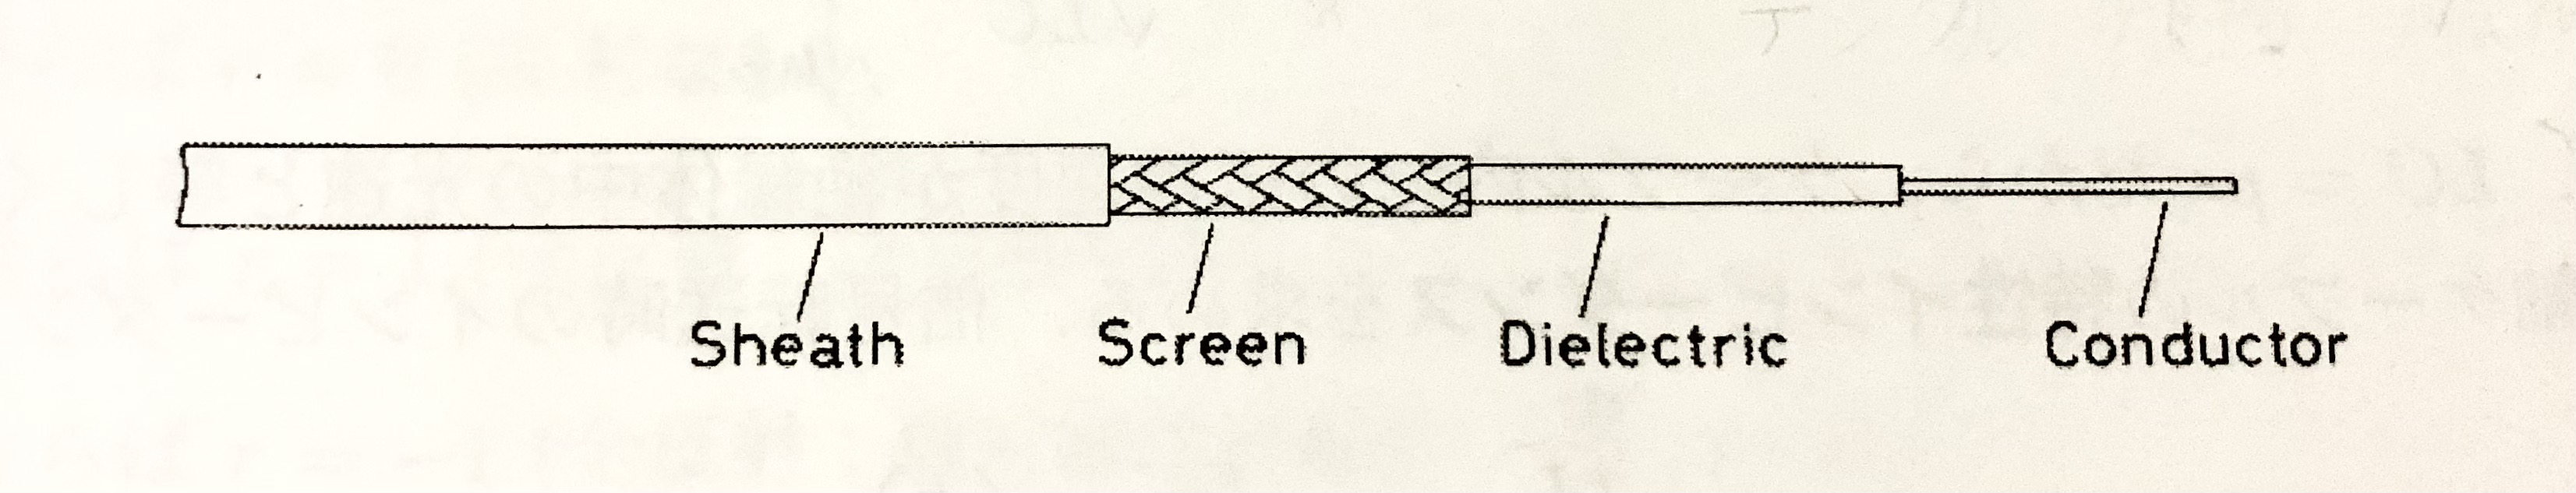
\includegraphics[width=14cm]{./assets/coaxial_cable.jpg}
  \caption{終端抵抗}
  \label{fig:coaxial cable}
\end{figure}
\begin{table}
  \centering
  \begin{tabular}{|c|l|}
    \hline
    構成部品       & 説明                \\
    \hline \hline
    Conductor  & 芯線と呼ばれる信号を流す導体    \\
    Dielectric & ポリエチレンやテフロンなどの絶縁体 \\
    Screen     & 同心円筒上に取り囲む外部導体    \\
    Sheath     & プラスチックのシールド       \\
    \hline
  \end{tabular}
  \caption{同軸ケーブルの構成}
  \label{table:coaxial cable}
\end{table}

同軸ケーブルの回路的側面の性質として芯線の半径を $a$、シールドの半径を $b$ とし、同軸ケーブルの静電容量 $C$ とインダクタンス $L$、並びに特性インピーダンス $Z_0$ と位相速度 $v$ は次のようになる。
\begin{align}
  C   & = \frac{2\pi\varepsilon}{\ln(b/a)} \sim \frac{55.6\varepsilon_r}{\ln(b/a)} \simeq 100 \si{pF/m}  \\
  L   & = \frac{\mu}{2\pi}\ln\frac{b}{a} \sim 0.2\mu_r\ln\frac{b}{a} \simeq 0.2 \si{\mu H/m}             \\
  Z_0 & = \sqrt{\frac{L}{C}} \sim 60\sqrt{\frac{\mu_r}{\varepsilon_r}}\ln\frac{b}{a} \simeq 50 \si{\ohm} \\
  v   & = \frac{\omega}{k} = \frac{1}{\sqrt{LC}} = \frac{1}{\sqrt{\mu\varepsilon}} = c
\end{align}
市販されている最も標準的なケーブル $b/a \simeq 3.6$, $\varepsilon_r \simeq 2.3$, $\mu_r = 1$ として計算した。

信号を正しく伝送するときに重要なこととしてインピーダンス整合が挙げられる。
インピーダンス整合とは同軸ケーブルの特性インピーダンスと終端抵抗を合わせることである。
インピーダンス整合をしていないと反射が起きる。その比率として電圧反射率 $r$ は次のように与えられる。
\begin{align}
  r = \frac{V_r}{V_0} = \frac{Z_L - Z_0}{Z_L + Z_0}
\end{align}



\section{実験手法}
今回行う実験における実験手法を説明する。
まず今回の実験で使う実験装置について観測部分と情報処理部分に分けて紹介する。

観測部分では $\gamma$ 線や宇宙線がシンチレータに入ることでシンチレーション光が発せられ、MPPC でそれを観測する。
シンチレータは基本的に無機シンチレータである GAGG 結晶を用い、比較としてプラスチックシンチレータである p-テルフェニルも用いる。
MPPC については $3\si{mm}\times 3\si{mm}$ の SN:68219 と $6\si{mm}\times 6\si{mm}$ の No.89-91 を用いる。

情報処理部分では観測部分で得られた信号を整形してオシロスコープや PC で表示する。
アンプで増幅や整形し、ディスクリミネータやコインシデンスで不要な情報をフィルタする。
実験装置の機器は表 \ref{table:machine} のものを用いた。
\begin{table}
  \centering
  \begin{tabular}{|clp{7cm}|}
    \hline
    実験装置         & 機器名                & 説明                          \\
    \hline \hline
    MPPC         & No.89-91, SN:68219 & 光検出器の一種。                    \\
    無機シンチレータ     & GAGG               & シンチレータの一種。                  \\
    プラスチックシンチレータ & p-テルフェニル           & シンチレータの一種。                  \\
    HV 電源        & Agilent E3612A     & 電圧を掛ける装置。                   \\
    アンプ          & Phillips 777       & 入力信号を増幅させて出力する。             \\
    SiPM プリアンプ   & Model 5035         & 入力信号を増幅させて出力する。             \\
    波形整形アンプ      & ORTEC 571          & あるゲイン以上のパルス波を整形された正弦波に変換する。 \\
    ディスクリミネータ    & -                  & あるゲイン以下のパルスをカットする。          \\
    コインシデンス      & -                  & 複数の入力がすべて上がっているときに出力される回路。  \\
    AD コンバータ     & CP 1114A           & アナログからデジタルへ変換する。            \\
    スケーラー        &                    &                             \\
    \hline
  \end{tabular}
  \caption{実験装置の機器名}
  \label{table:machine}
\end{table}


\subsection{同軸ケーブル}
まず次のような手順で同軸ケーブル内の信号伝搬速度を調べる。
\begin{enumerate}
  \item パルス発生装置からオシロスコープの 1ch に繋げる。
  \item 同軸ケーブルの長さを測り, オシロスコープの 1ch から 2ch に繋げる。
  \item オシロスコープで 1ch と 2ch の位相差を調べる。
\end{enumerate}
次に以下の手順で信号の反射を調べる。
\begin{enumerate}
  \item パルス発生装置からオシロスコープの 1ch に繋げる。
  \item 3\si{m} の同軸ケーブルの端を抵抗でショートする。
\end{enumerate}
実験 1-(3) については何らかの故障により実験が行えなかった。


\subsection{MPPC のダークレート測定}
\begin{enumerate}
  \item $3\si{mm}\times 3\si{mm}$ の MPPC (SN:68219) を遮光し、HV に接続する。
  \item HV 電源を 72.7 \si{V} として HV 電源からアンプ、ディスクリミネータに繋いでオシロスコープで波形を観測する。
  \item ディスクリミネータのスレッショルドを 2-3 \si{mV} ずつ変えながらスケーラーで 30 秒間の計数を測定する。
\end{enumerate}


\subsection{$\gamma$ 線の計測}
ここではを用いて線源から出る $\gamma$ 線を検出する。

次のような手順で実験する。
\begin{enumerate}
  \item シンチレータに MPPC を貼り付け、気泡が入らないようにテフロンテープで巻く。
  \item シンチレータと MPPC をブラックシートで覆って遮光する。
  \item MPPC を HV 供給アダプタに繋げる。
  \item 電源を 40.2 V に設定して電源から HV 供給アダプタ, SiPM アンプ, 波形整形アンプ, AD コンバータ, PC の順に繋げる。
  \item PC で 5 分間、チャンネルに対応するパルス数を観測する。
\end{enumerate}
そうして得られたグラフによって光電ピークが見られるのでそれを用いてチャンネルとエネルギーの単位換算ができる。


\subsection{宇宙線の計測}
\begin{enumerate}
  \item プラスチックシンチレータに MPPC を貼り付けたものを 2 つ用意し上下に重ね、HV 供給アダプタの Ch1, Ch2 に繋げる。
  \item アンプ、ディスクリミネータ、コインシデンス、スケーラを繋げてパルス数を観測する。
\end{enumerate}



\section{実験結果}
\subsection{同軸ケーブル}
長さ $99.9\si{cm}$ の同軸ケーブルに対し、$5.8\si{ns}$ で信号が到達した。
\begin{figure}[htbp]
  \centering
  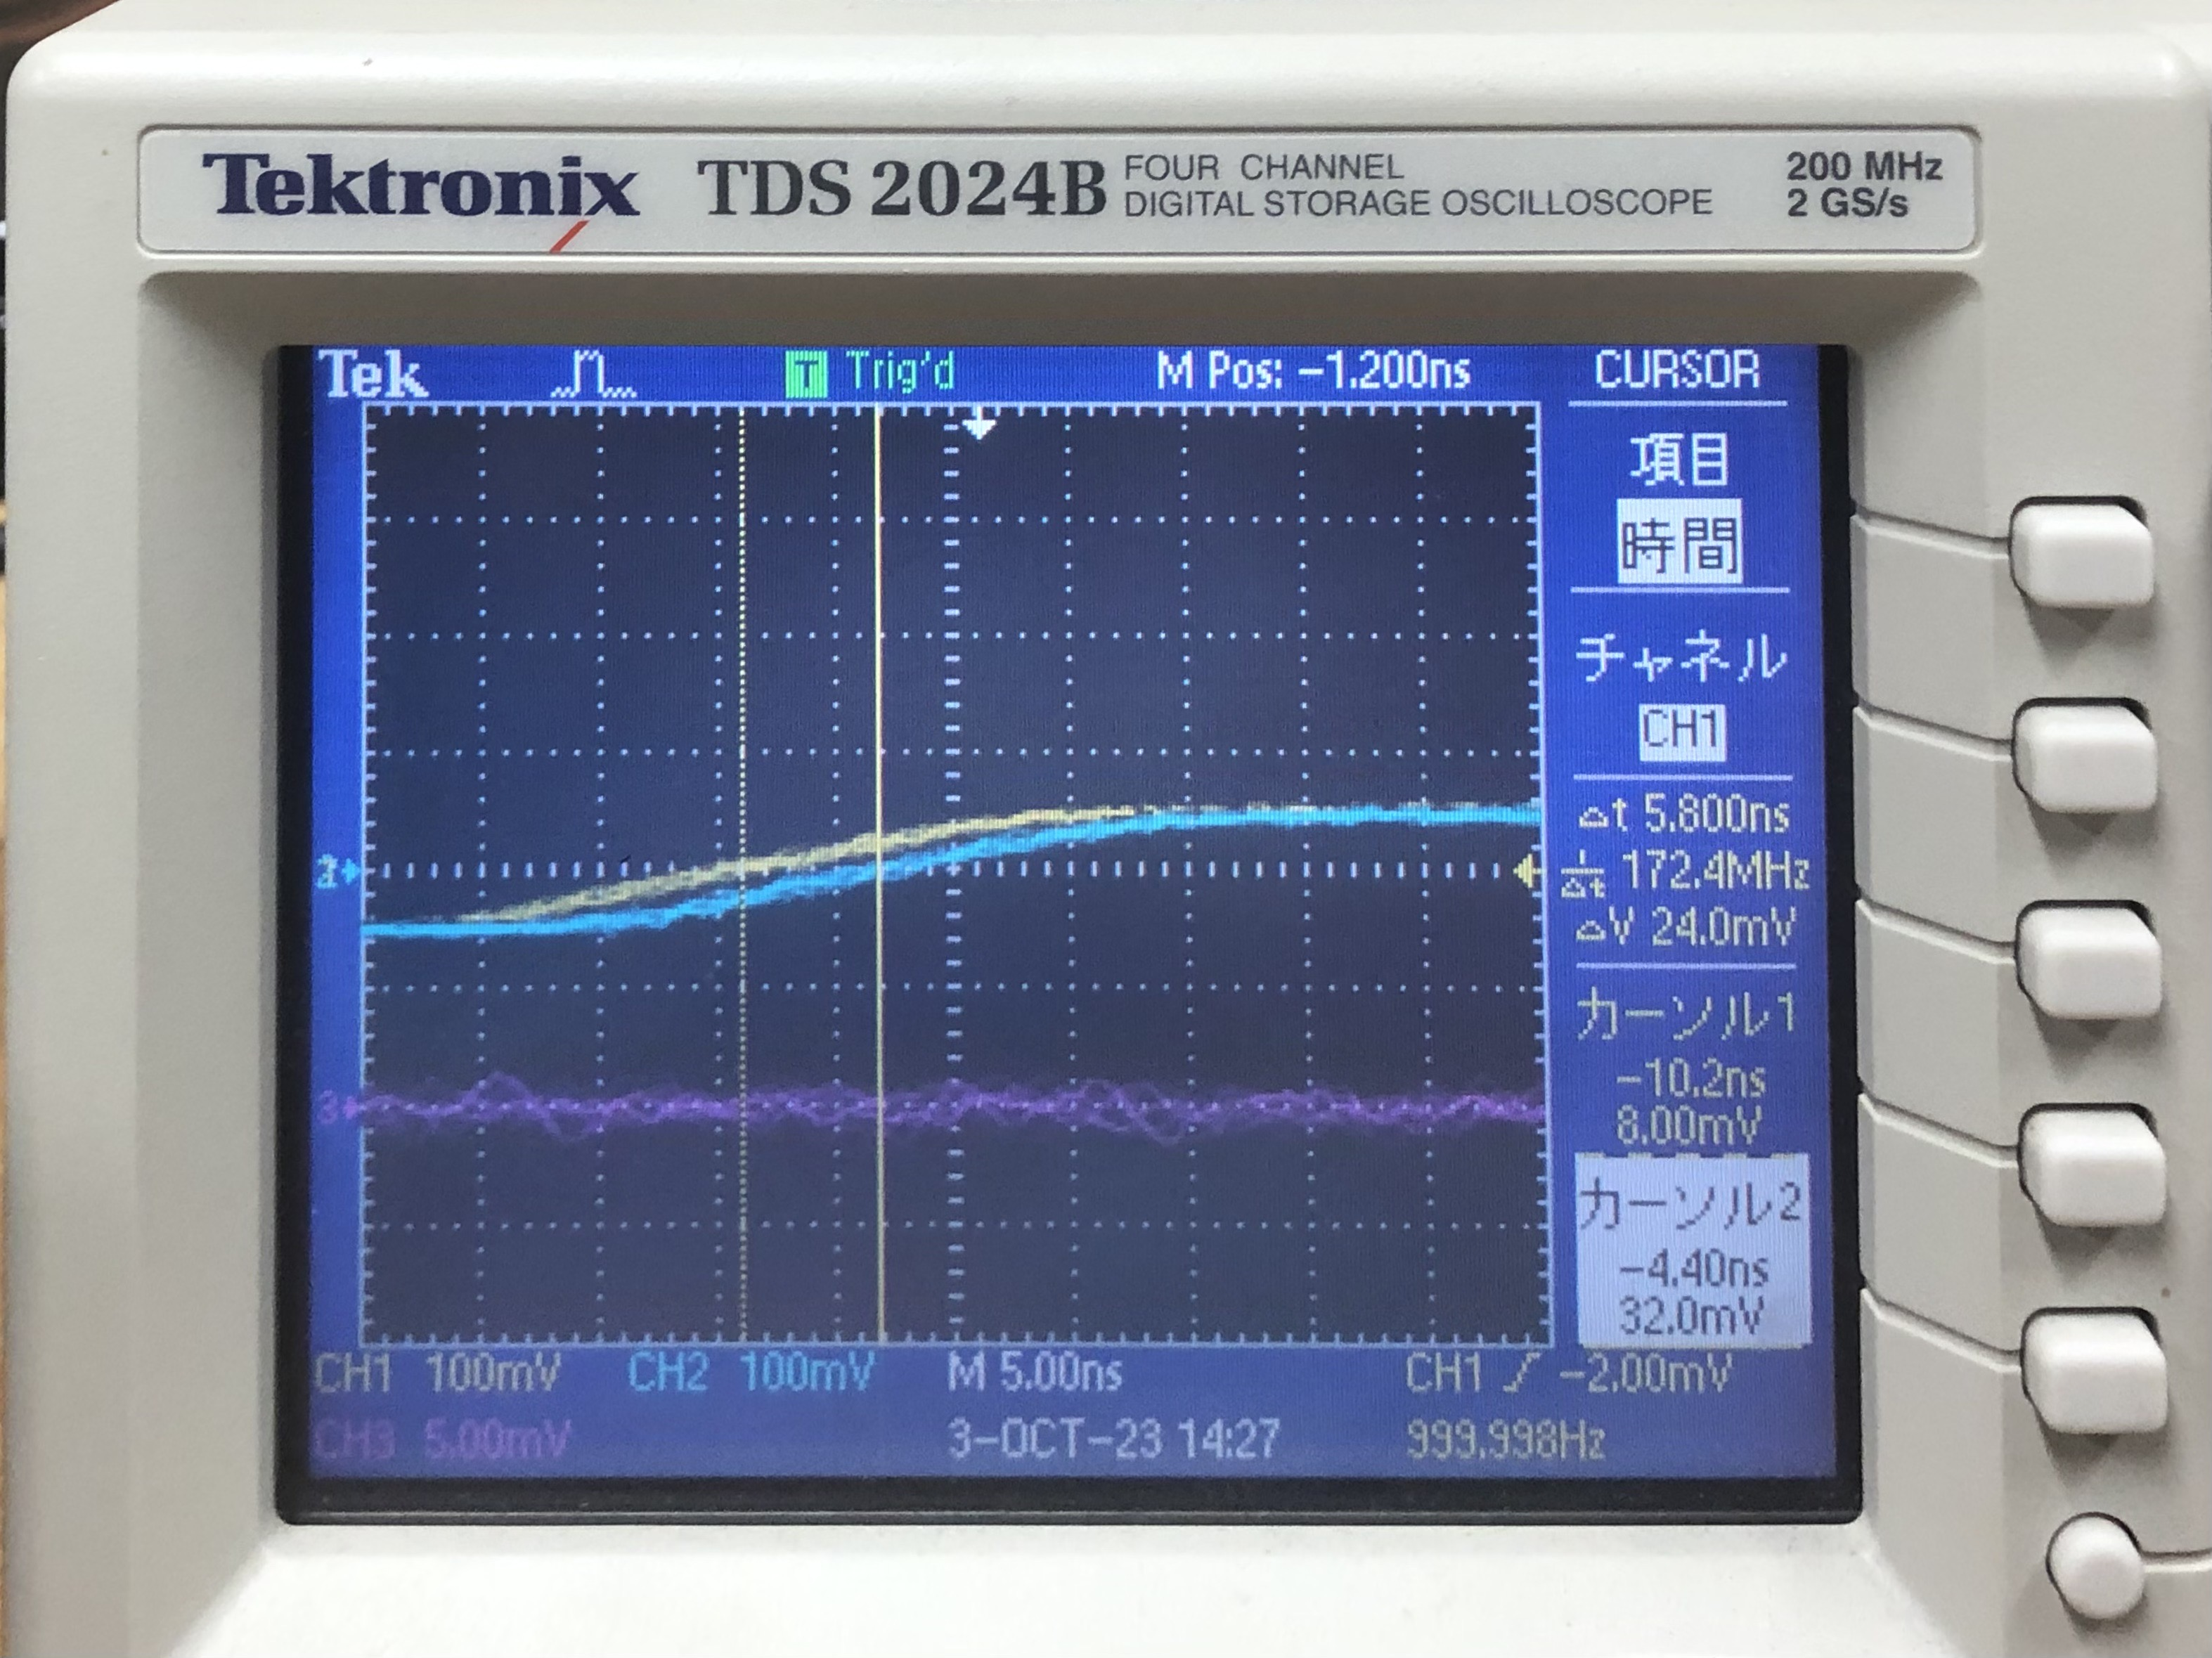
\includegraphics[width=10cm]{./assets/cable_diff_time.jpg}
  \caption{ケーブル}
  \label{fig:cable diff time}
\end{figure}

終端抵抗を変えたときのパルス波の強度は表 \ref{table:resistance} のようになり、パルス波の様子は図 \ref{fig:reflection} のようになった。
\begin{table}
  \centering
  \begin{tabular}{|c|c|}
    \hline
    終端抵抗値              & パルス波の強度     \\
    \hline
    1 \si{\ohm}        & 20 \si{mV}  \\
    50 \si{\ohm}       & 100 \si{mV} \\
    100 \si{\ohm}      & 130 \si{mV} \\
    $\infty$ \si{\ohm} & 200 \si{mV} \\
    \hline
  \end{tabular}
  \caption{終端抵抗に対するパルス波の強さ}
  \label{table:resistance}
\end{table}
\begin{figure}[htbp]
  \centering
  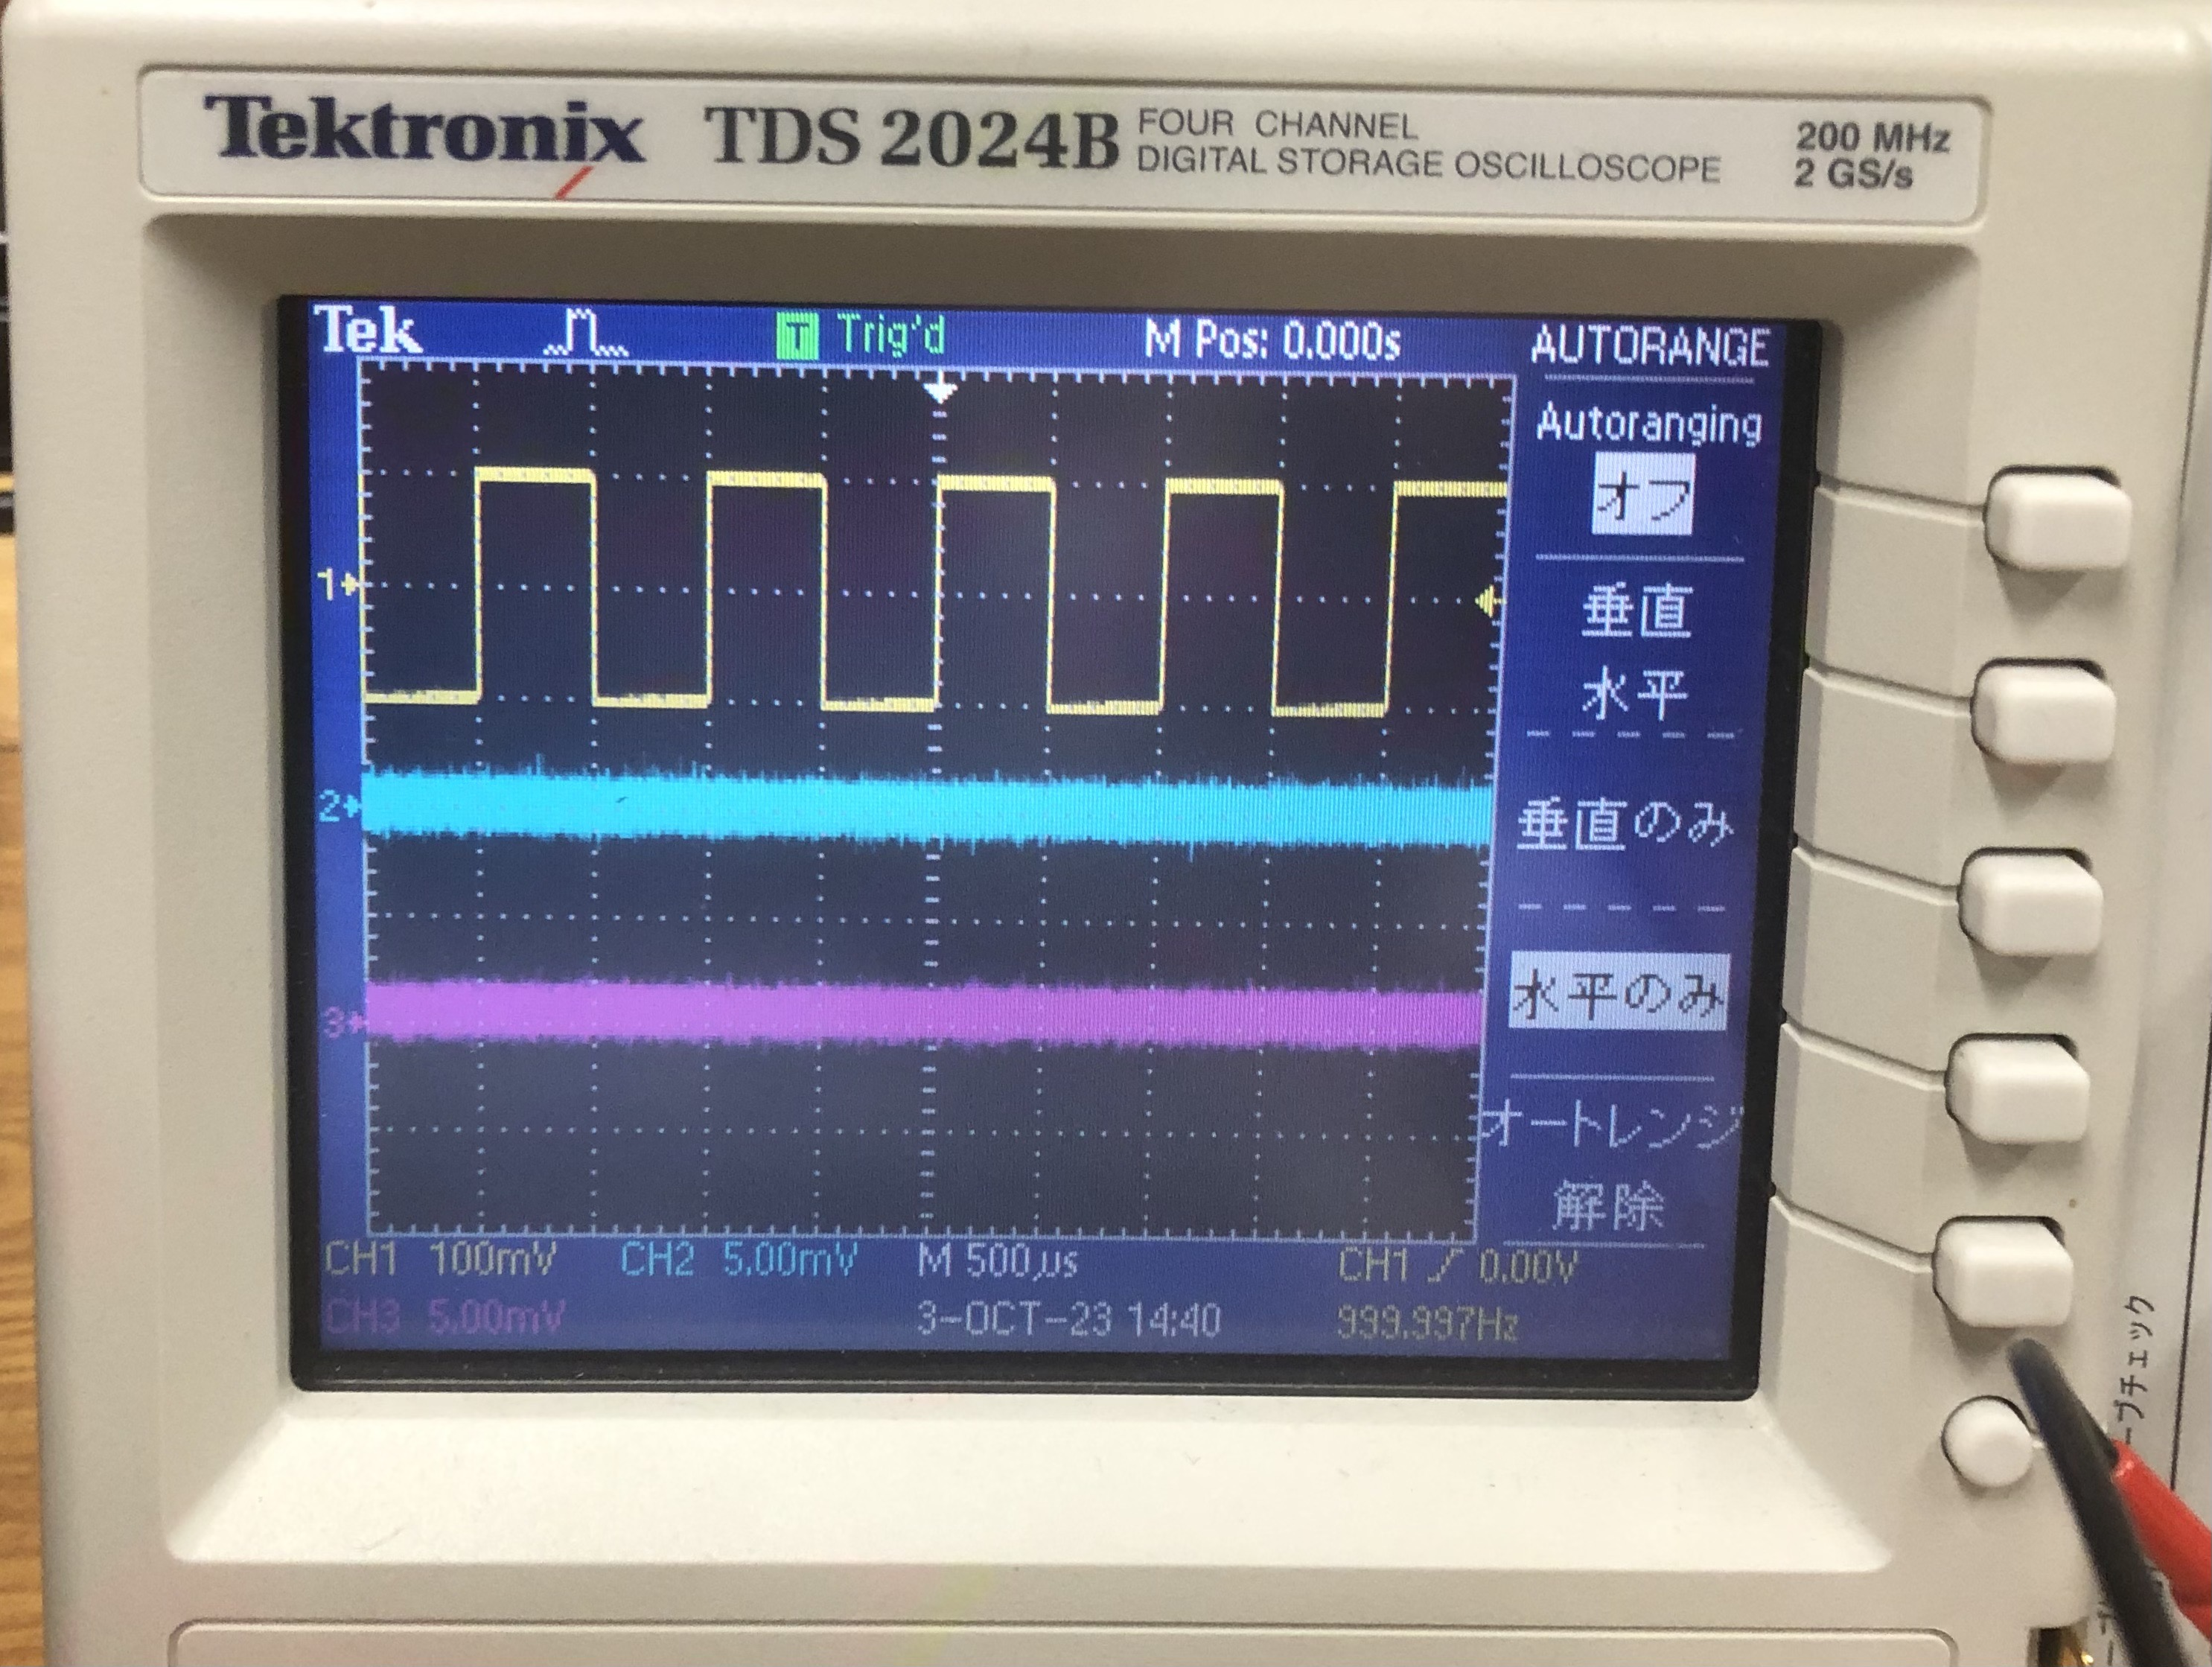
\includegraphics[width=10cm]{./assets/reflection.jpg}
  \caption{終端抵抗}
  \label{fig:reflection}
\end{figure}


\subsection{MPPC のダークレート測定}
ディスクリミネータの閾値を少しずつ変えて計数を比較する実験については図 \ref{fig:darkrate discriminator} のようになった。
\begin{figure}[htbp]
  \centering
  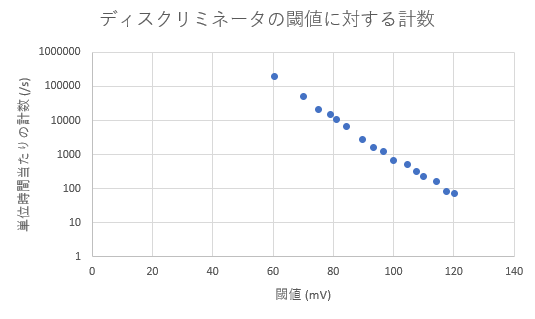
\includegraphics[width=12cm]{./assets/discriminator.png}
  \caption{ダークレートにおいて閾値に対する計数}
  \label{fig:darkrate discriminator}
\end{figure}

またオシロスコープでは図 \ref{fig:trigger 1} のような波形が見られた。
\begin{figure}[htbp]
  \centering
  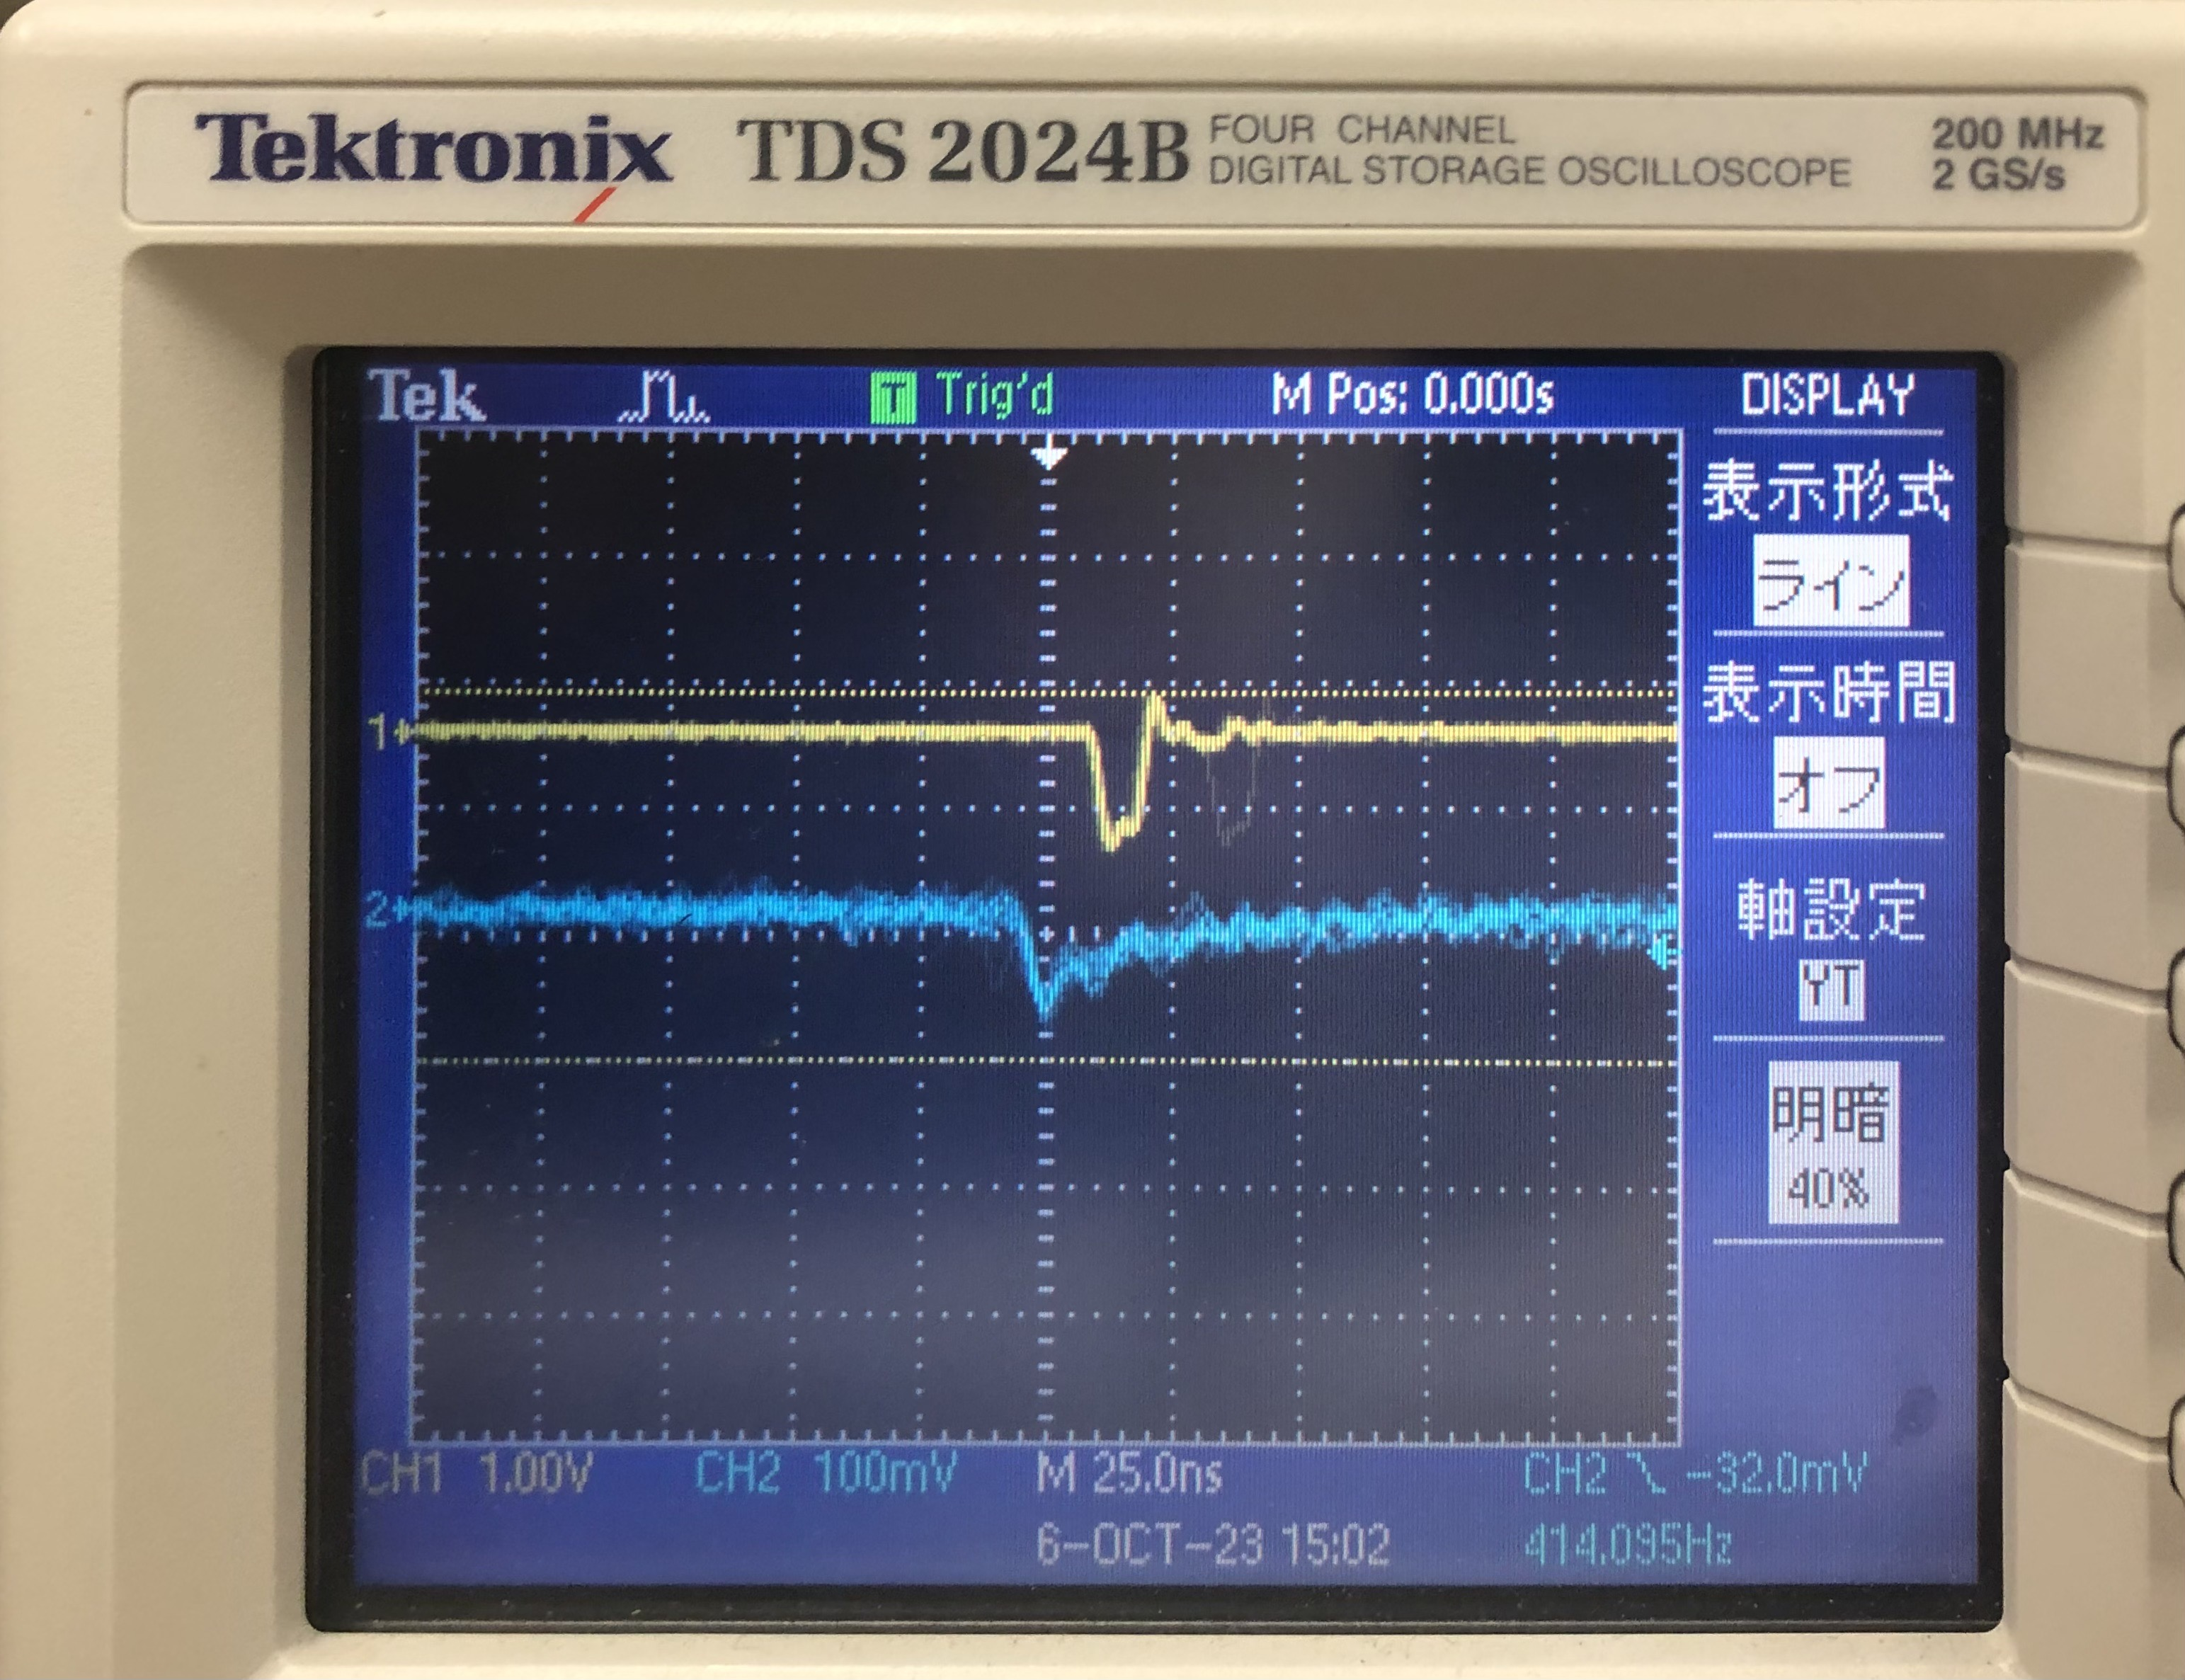
\includegraphics[width=12cm]{./assets/trigger1.jpg}
  \caption{ダークレート測定におけるオシロスコープの観察}
  \label{fig:trigger 1}
\end{figure}


\subsection{$\gamma$ 線の計測}
線源 \ce{Co^60}, \ce{Na^22}, \ce{Cs^137}, \ce{Ba^133} のガンマ線の計測結果をそれぞれ図 \ref{fig:Co60 gamma}, \ref{fig:Na22 gamma}, \ref{fig:Cs137 gamma}, \ref{fig:Ba133 gamma} に示す。
\begin{figure}[htbp]
  \centering
  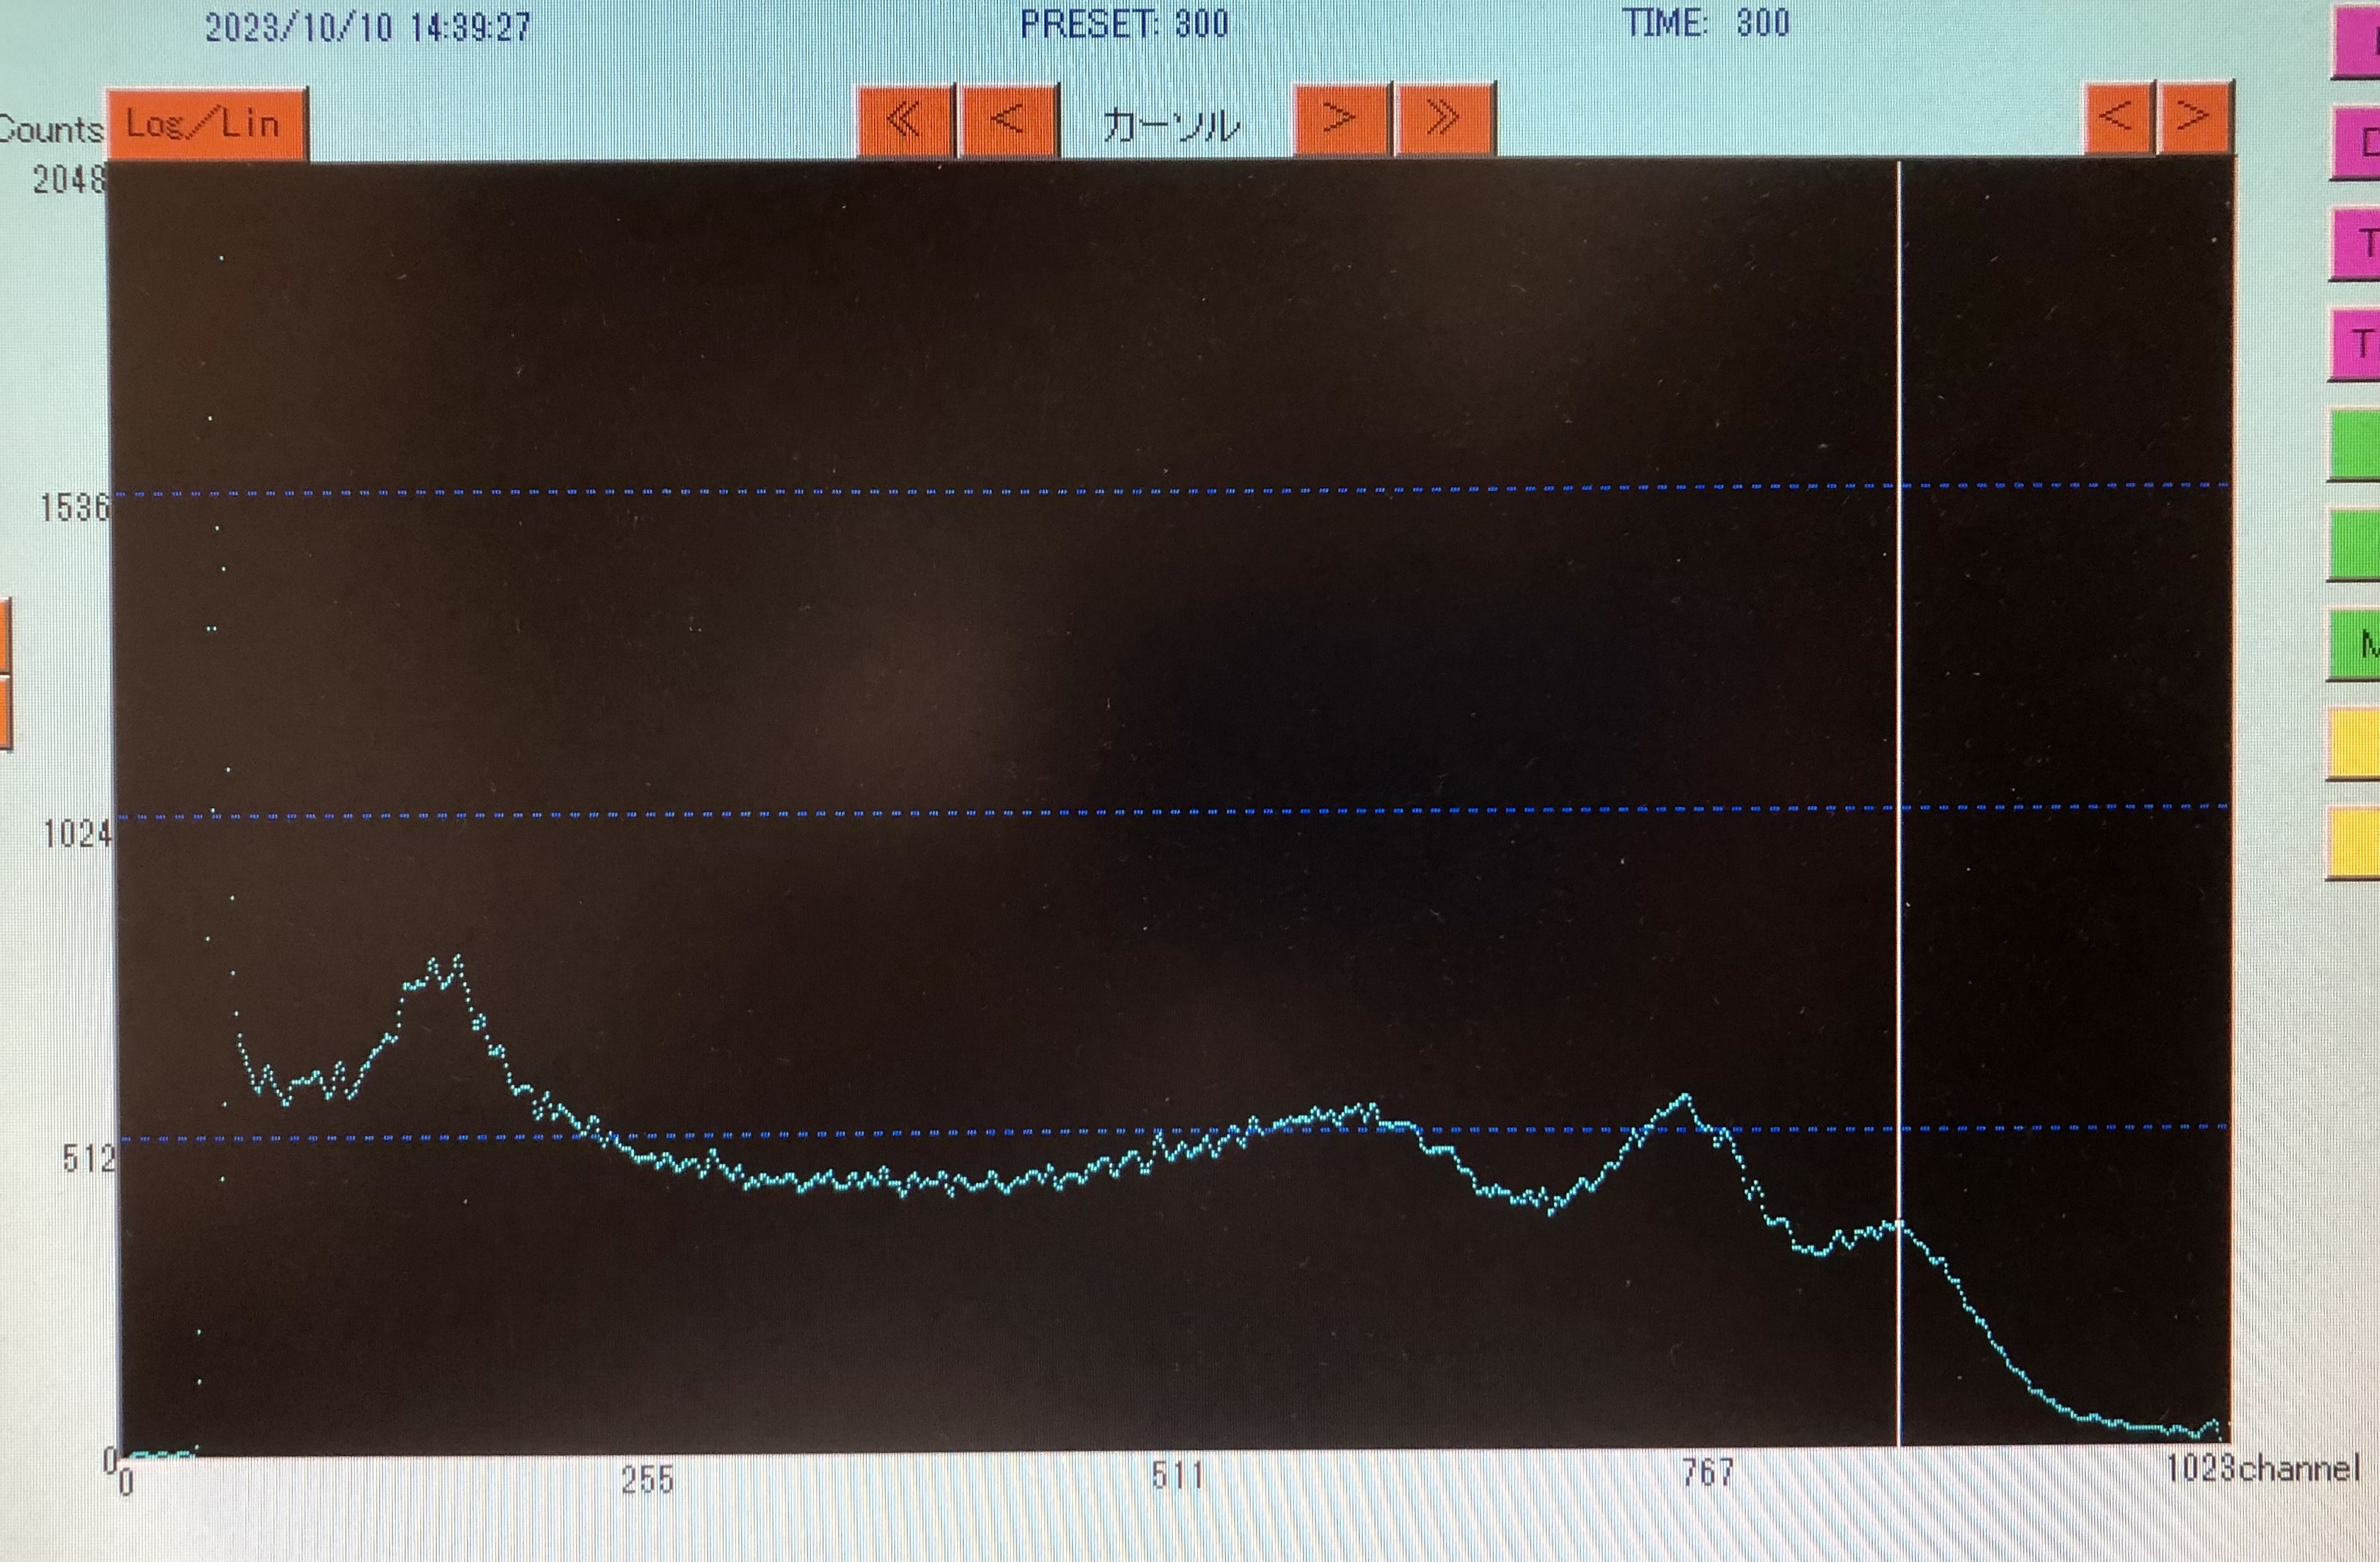
\includegraphics[width=14cm]{./assets/Co60_gamma.jpg}
  \caption{線源 \ce{Co^{60}} のガンマ線の計測結果}
  \label{fig:Co60 gamma}
\end{figure}
\begin{figure}[htbp]
  \centering
  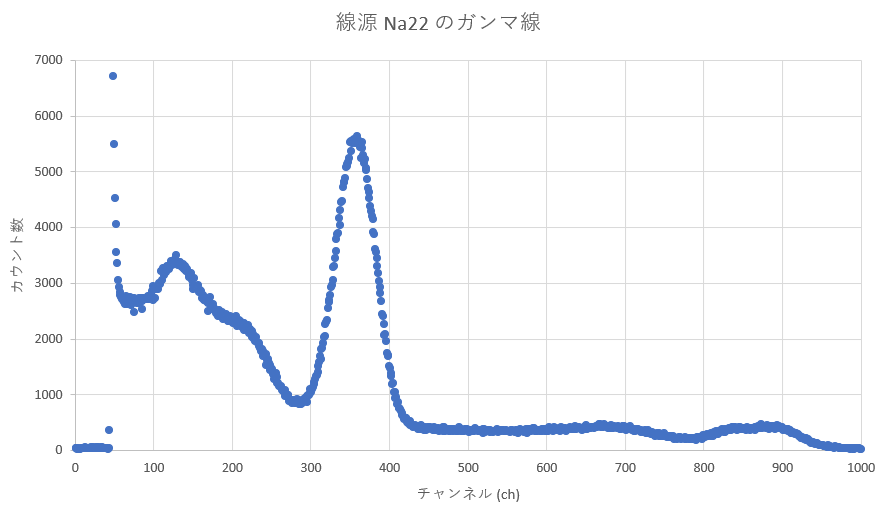
\includegraphics[width=12cm]{./assets/Na22_gamma.png}
  \caption{線源 \ce{Na^22} のガンマ線の計測結果}
  \label{fig:Na22 gamma}
\end{figure}
\begin{figure}[htbp]
  \centering
  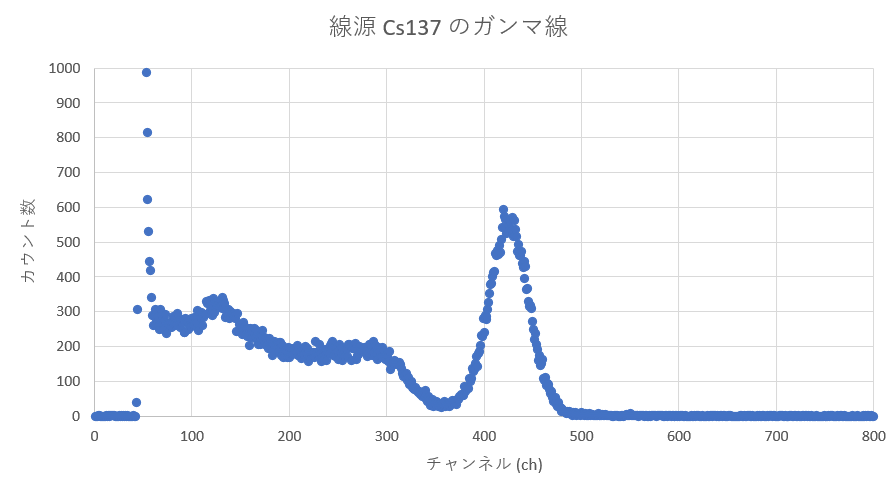
\includegraphics[width=12cm]{./assets/Cs137_gamma.png}
  \caption{線源 \ce{Cs^137} のガンマ線の計測結果}
  \label{fig:Cs137 gamma}
\end{figure}
\begin{figure}[htbp]
  \centering
  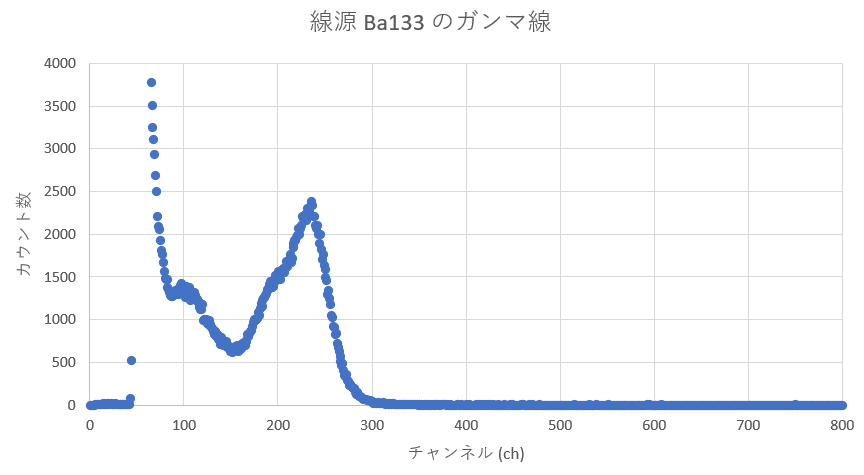
\includegraphics[width=12cm]{./assets/Ba133_gamma.png}
  \caption{線源 \ce{Ba^133} のガンマ線の計測結果}
  \label{fig:Ba133 gamma}
\end{figure}
\begin{figure}[htbp]
  \centering
  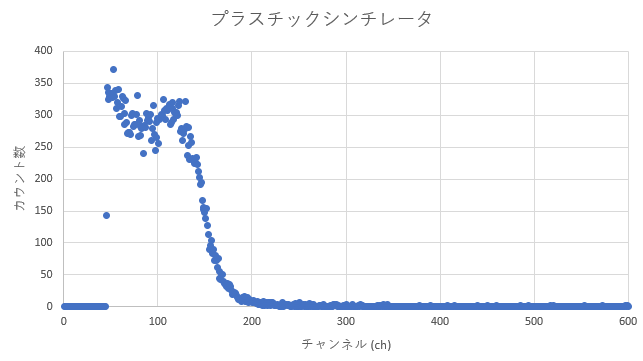
\includegraphics[width=12cm]{./assets/plastic.png}
  \caption{線源 \ce{Ba^133} のガンマ線のプラスチックシンチレータによる計測結果}
  \label{fig:Ba133 plastic}
\end{figure}

またオシロスコープでは図 \ref{fig:trigger 2} のような波形が見られた。
\begin{figure}[htbp]
  \centering
  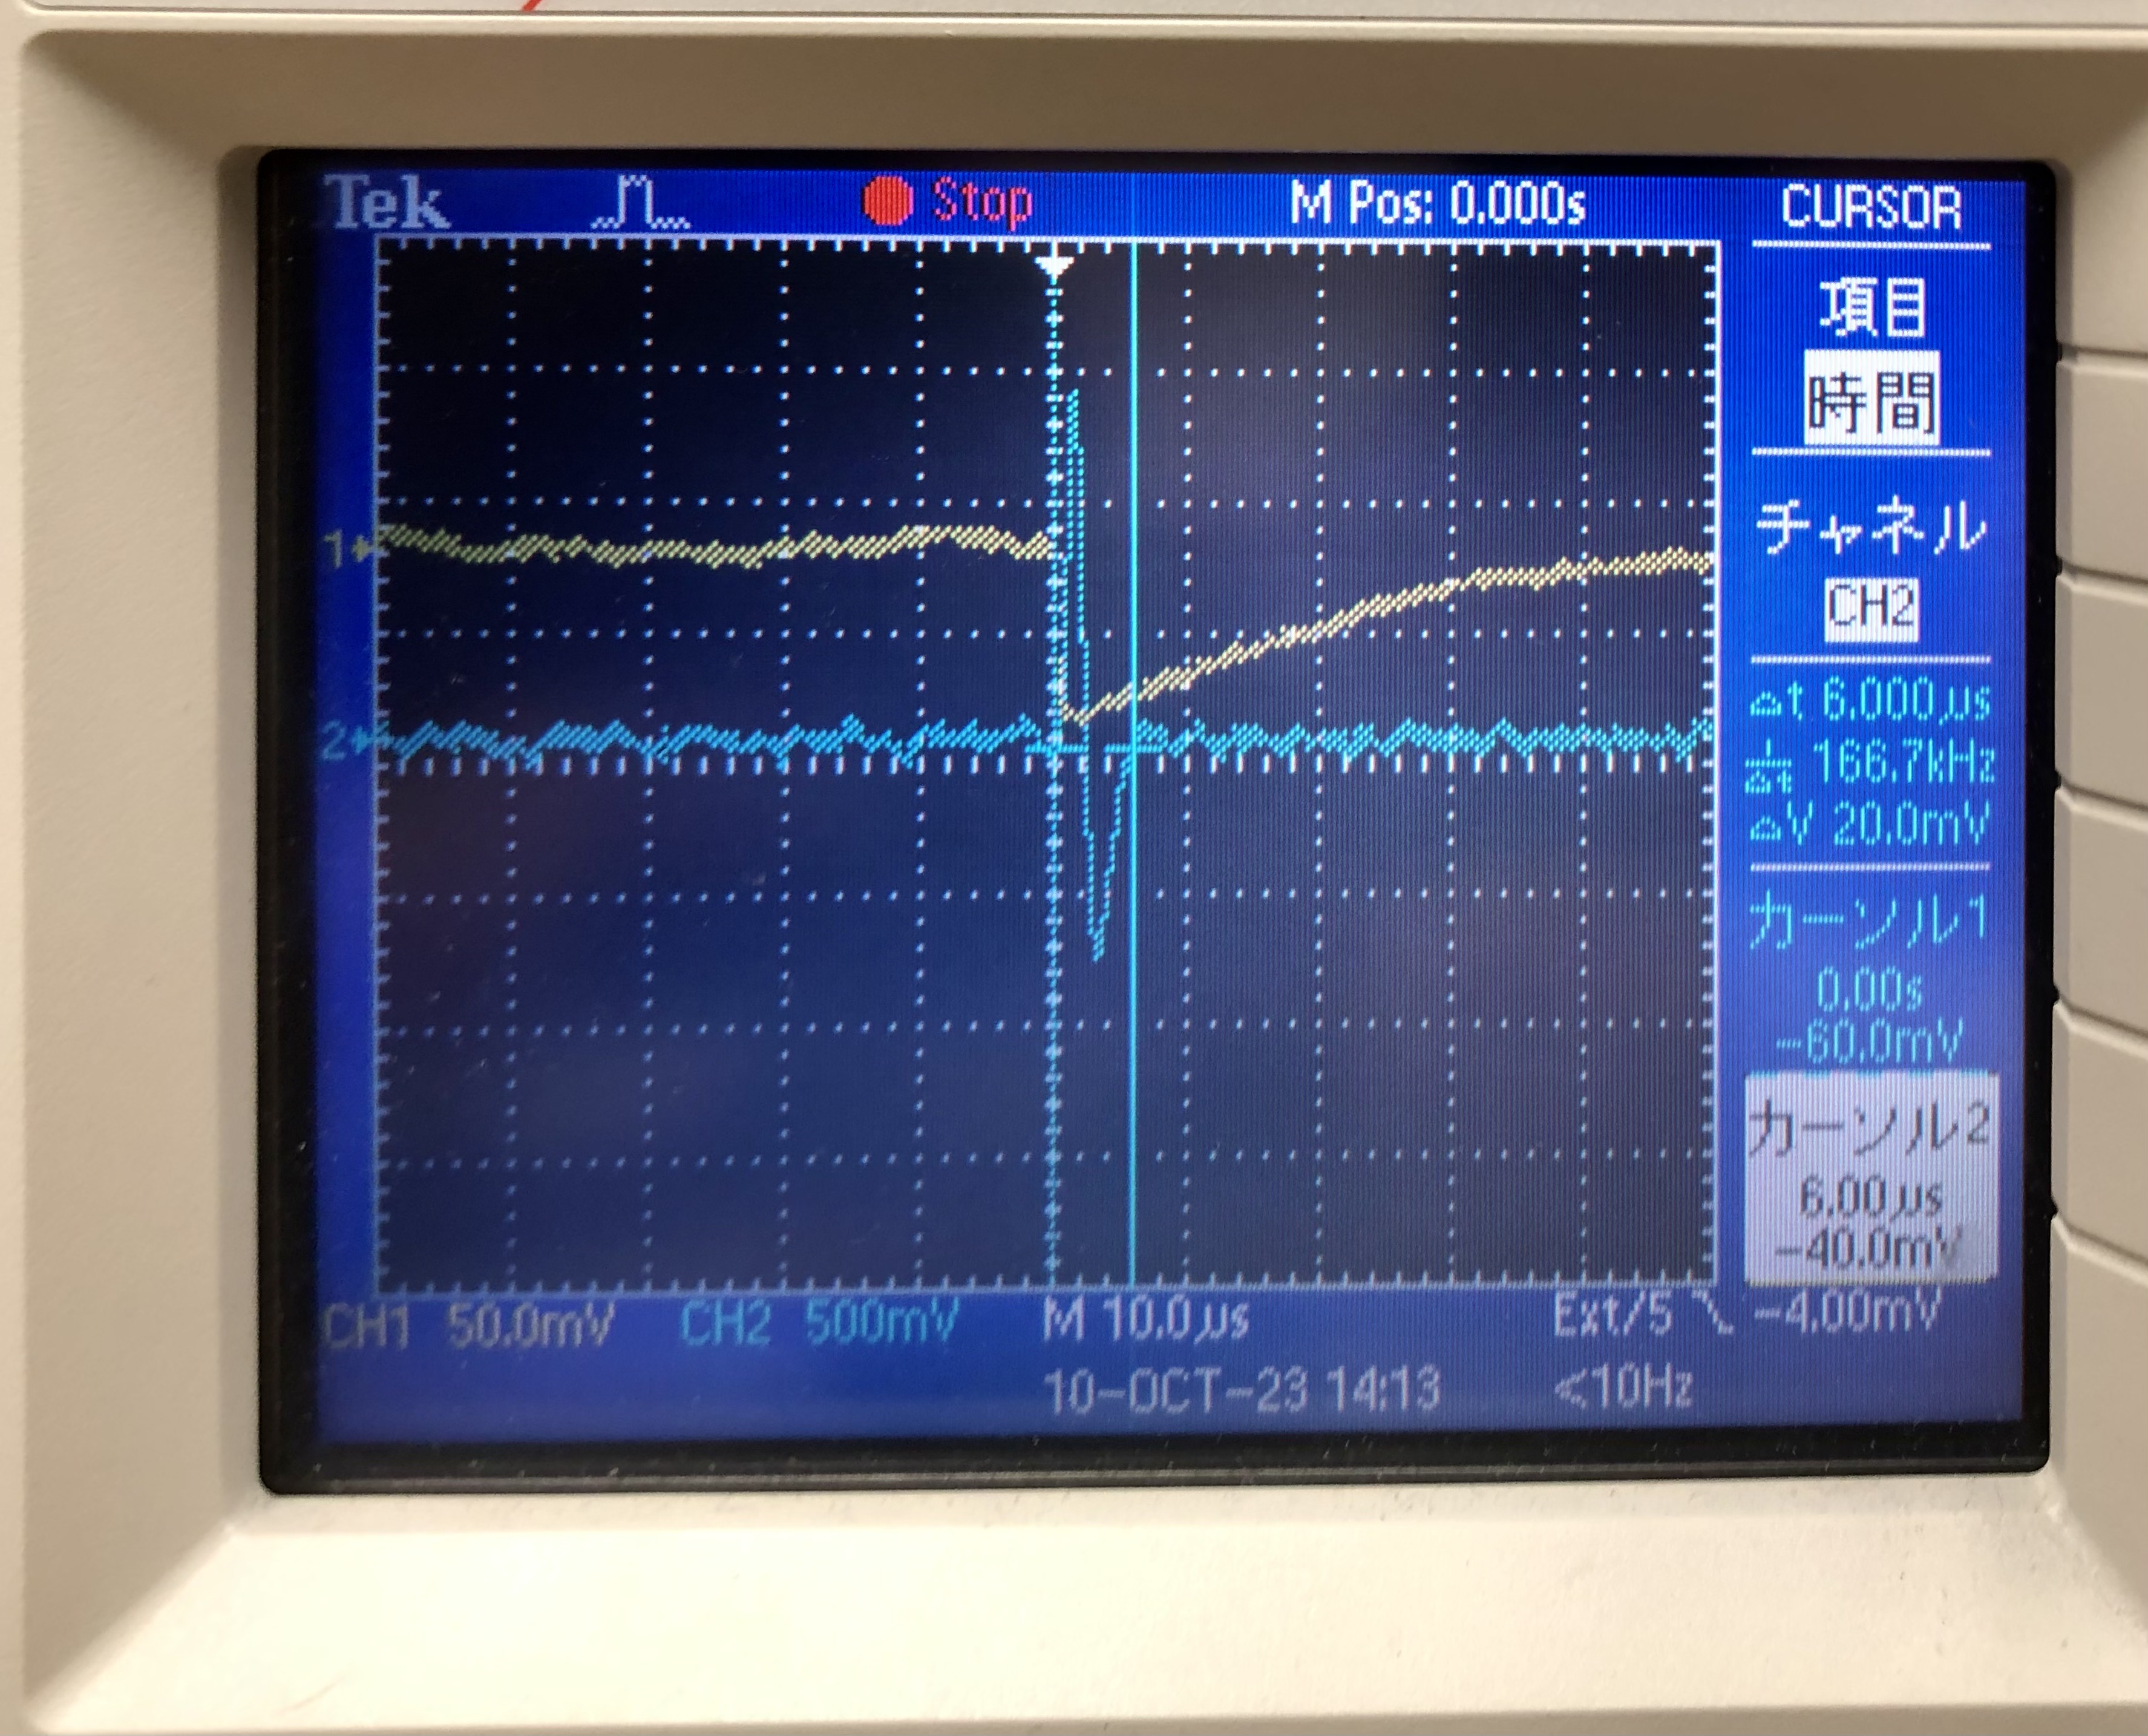
\includegraphics[width=12cm]{./assets/trigger2.jpg}
  \caption{$\gamma$ 線の計測におけるオシロスコープの観察}
  \label{fig:trigger 2}
\end{figure}


\subsection{宇宙線の計測}
$40\si{mm}\times 40\si{mm}$ のシンチレータに対して平均毎分 14.7 個の宇宙線が観測された。
また 2 つのシンチレータを十分離すと宇宙線が観測されなくなった。
\begin{figure}[htbp]
  \centering
  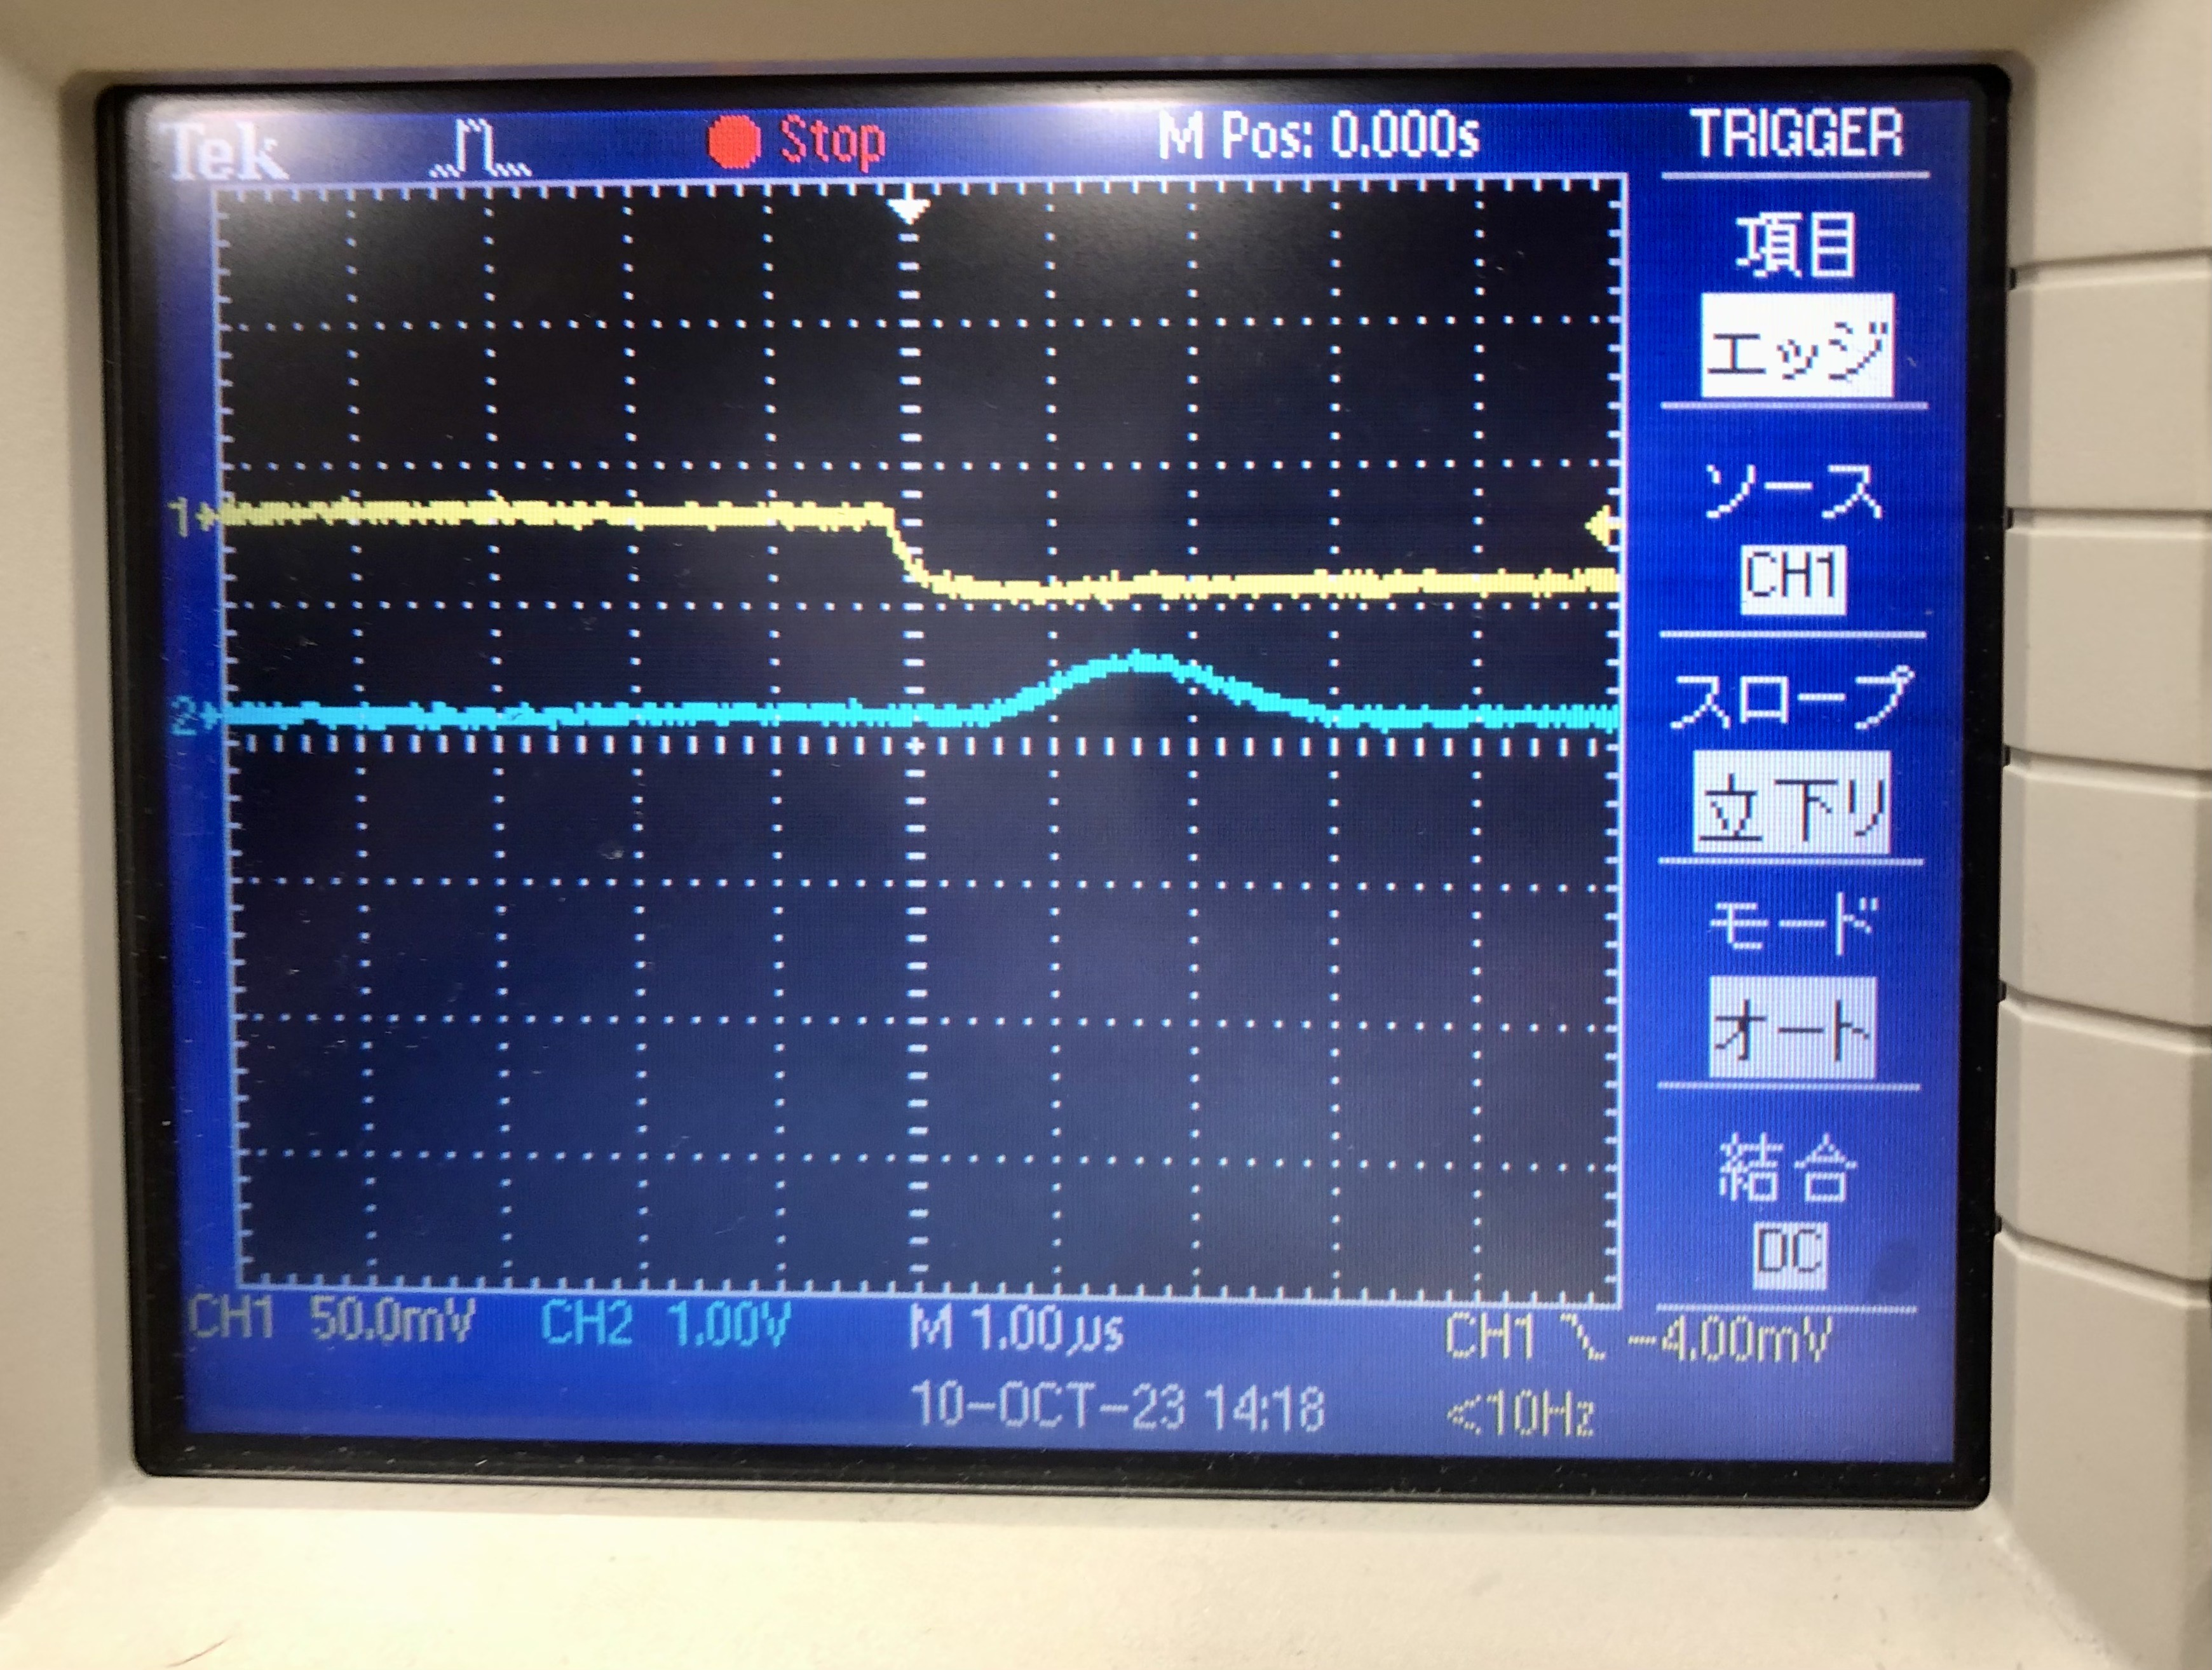
\includegraphics[width=12cm]{./assets/trigger3.jpg}
  \caption{宇宙線の計測におけるオシロスコープの観察}
  \label{fig:trigger 3}
\end{figure}
仰角に対する宇宙線は図 \ref{fig:cosmic ray angle} のように観測された。
\begin{figure}[htbp]
  \centering
  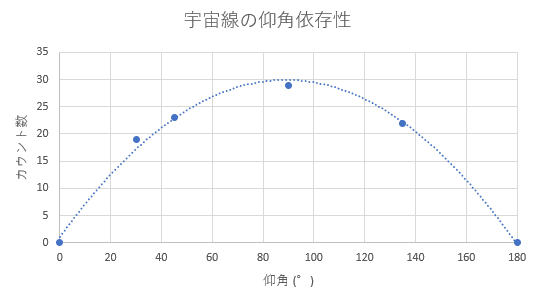
\includegraphics[width=14cm]{./assets/cosmic_ray_elevation_angle.png}
  \caption{宇宙線の天頂角分布}
  \label{fig:cosmic ray angle}
\end{figure}



\section{考察}
\subsection{同軸ケーブル}
同軸ケーブルの長さは $99.9\si{cm}$ に対し、$5.8\si{ns}$ で信号到達したことから信号伝達速度は次のようになる。
\begin{align}
  \frac{99.9\si{cm}}{5.8\si{ns}} \approx 1.72\times 10^5\si{km/s}
\end{align}
これは光速の約 $57\%$ である。同軸ケーブルの信号伝搬速度は光速であるからオーダーとしては一致している。

特性インピーダンスが $Z_0 = 50\si{\ohm}$ の同軸ケーブルの終端抵抗 $Z_L$ を変更すると次のように電圧反射率 $r$ が変動する。
\begin{align}
  r & = \frac{V_r}{V_0} = \frac{Z_L - Z_0}{Z_L + Z_0} = \begin{cases}
                                                          -0.96 & (1 \si{\ohm})      \\
                                                          0     & (50 \si{\ohm})     \\
                                                          0.33  & (100 \si{\ohm})    \\
                                                          1     & (\infty \si{\ohm}) \\
                                                        \end{cases}
\end{align}
これより $100 \si{mV}$ に対してそれぞれ 4 \si{mV}, 100 \si{mV}, 133 \si{mV}, 200 \si{mV} となる。
これは 1 \si{\ohm} の終端抵抗以外は実験結果と一致している。
この違いの具体的な原因は消去法としてオシロスコープのインピーダンスによるものと思われる。
オシロスコープのインピーダンスにより位相などのパラメータが変化し 4 \si{\ohm} 程度の余分なインピーダンスが入ってしまったと考えられる。


\subsection{MPPC のダークレート測定}
図 \ref{fig:darkrate discriminator} の対数グラフを見ると大方直線となっているのに対して 25 \si{mV} 毎に上下していることが分かる。
これにはクロストークが原因であると考えられる。
すべてが 1 回の入射に対して 25 \si{mV} 程度出るのであればクロストークによりその倍数だけ観測される。
これによりグラフが階段状になると考えられる。
その性質が顕著には現れなかったのはノイズが多く正確に測れなかったからだと考えられる。


\subsection{$\gamma$ 線の計測}
観測した光電ピークとチャンネルとエネルギーの対応が分かっているので図 \ref{fig:energy ch} のように線形近似して関係式を導ける。
\begin{figure}[htbp]
  \centering
  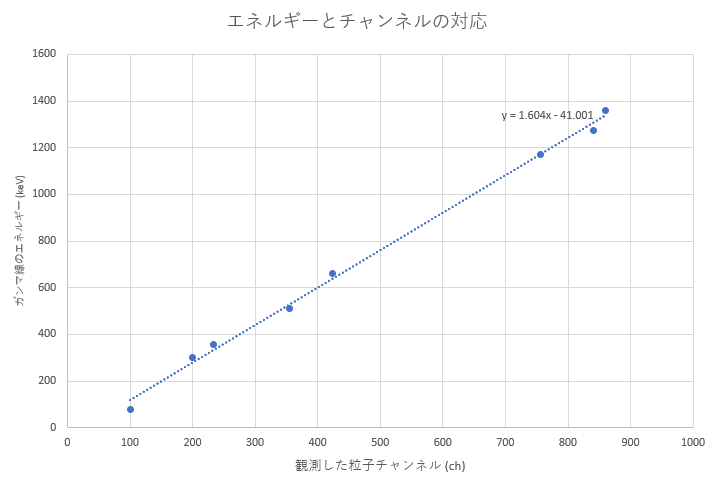
\includegraphics[width=14cm]{./assets/gamma_energy_ch.png}
  \caption{エネルギーとチャンネルの対応}
  \label{fig:energy ch}
\end{figure}

これより表 \ref{table:peak} のようなピークが観測された。
\begin{table}
  \centering
  \begin{tabular}{|c|lp{5cm}|}
    \hline
    線源 & 観測されたピーク (keV)                        & 理論的な光電ピーク (keV) \\
    \hline \hline
    Co & 215.6, 921.4, 1172, 1338              & 1170, 1360      \\
    Cs & 157.9, 419.3, 637.5                   & 662             \\
    Na & 162.7, 303.9, 528.4, 1034, 1306, 1385 & 1274            \\
    Ba & 119.4, 279.8, 334.3                   & 80, 303, 356    \\
    \hline
  \end{tabular}
  \caption{ガンマ線のピーク位置}
  \label{table:peak}
\end{table}

光電効果による光電ピークに対してコンプトン散乱とその後方散乱のピークのエネルギー和が等しくなっていることがわかる。また \ce{Na^22} では 511 \si{keV} の $\beta^+$ 崩壊による陽電子と電子の電子対消滅による $\gamma$ 線が出ていることが分かる。
プラスチックシンチレータについては正しくエネルギーを変換できておらず $\gamma$ 線には向いていないという資料の内容と一致していることが分かる。


\subsection{宇宙線の計測}
今回観測した量は $1\si{\cm^2}$ 当たりに換算すると $0.91\si{count/cm^2\cdot s}$ と $1$ に近く資料と一致している。
また宇宙線は天頂に近いほど多く観測されたことに関しては $\mu$ 粒子は大気によって指数的に減衰するということを示唆していると考えられる。



\section{レポート問題}
\subsection{基礎問題}
\begin{problem}[準備 1]
$\hbar c = 197\si{MeV\cdot fm}$ であることを確かめよ。1 \si{GeV} のフォトンの波長を調べよ。
\end{problem}
\begin{proof}
  \begin{align}
    \hbar c & \approx (6.582 \times 10^{-16} \si{eV\cdot s}) \times (2.998\times 10^8 \si{m/s}) \\
            & \approx 1.973\times 10^{-7}\si{eV\cdot m}                                         \\
            & \approx 197.3\ \si{MeV\cdot fm}
  \end{align}
  \begin{align}
    E       & = \frac{hc}{\lambda}                                                                      \\
    \lambda & = \frac{2\pi\hbar c}{E} = \frac{6.28\times 197\si{MeV\cdot fm}}{1 \si{GeV}} = 1.24\si{fm}
  \end{align}
  よって波長は $1.24\si{fm}$ となる。
\end{proof}

\begin{problem}
特殊相対論の次の式を用いて $\beta, \gamma, \gamma\beta$ を計算せよ。
\begin{align}
  E^2 - (pc)^2 & = (mc^2)^2, \qquad p = \frac{Ev}{c^2}
\end{align}
\end{problem}
\begin{proof}
  \begin{align}
    \beta       & := \frac{v}{c} = \frac{pc}{E}                                                               \\
    \gamma      & := \frac{1}{\sqrt{1 - \beta^2}} = \frac{1}{\sqrt{1 - \ab(\frac{pc}{E})^2}} = \frac{E}{mc^2} \\
    \gamma\beta & = \frac{p}{mc}
  \end{align}
\end{proof}

\begin{problem}
2.2\si{\mu s} で崩壊する $\mu$ 粒子がなぜ地表 20 \si{km} に到達するのか?
ただし静止質量 105.6 \si{MeV/c^2}, 運動量 3 \si{GeV/c} とする。
\end{problem}
\begin{proof}
  \begin{align}
    E      & = \sqrt{(mc^2)^2 + (pc)^2} = \sqrt{(105.6 \si{MeV})^2 + (3 \si{GeV})^2} = 3.001858 \si{GeV} \\
    \gamma & = \frac{E}{mc^2} = 28.43
  \end{align}
  よって $2.2\si{\mu s}$ で $660\si{m}\times\gamma = 18.8\si{km}$ まで進めることが分かる.
\end{proof}

\begin{problem}
2 個の電子を無限遠方から徐々に近づけると静電ポテンシャルが徐々に増加していき, 静電ポテンシャルが電子の質量エネルギー $m_ec^2$ に等しくなるとき古典電子半径に一致することを示せ。$4\pi r_e^2$ が 1\si{barn} に一致することを示せ。
\end{problem}
\begin{proof}
  2 個の電子を無限遠方から徐々に近づけると静電ポテンシャルが徐々に増加していき, 静電ポテンシャルが電子の質量エネルギー $m_ec^2$ に等しくなるとき
  \begin{align}
     & \frac{e^2}{4\pi\varepsilon_0 r} = m_ec^2 \\
     & r = \frac{e^2}{4\pi\varepsilon_0m_ec^2}
  \end{align}
  より電子間の距離 $r$ は古典電子半径 $r_e$ に一致する. そして次のように計算できる。
  \begin{align}
    r_e        & = \frac{e^2}{4\pi\varepsilon_0m_ec^2} \approx \frac{(1.602\times 10^{-19}\si{C})^2}{12.56\times(8.85\times 10^{-12}\si{F/m})\times(8.19\times 10^{-14}\si{J})} = 2.818 \times 10^{-15}\si{m} \\
    4\pi r_e^2 & \approx 0.998 \times 10^{-28}\si{m^2} = 10^{-24}\si{cm^2} = 1\si{barn}
  \end{align}
\end{proof}


\subsection{MPPC の原理}
ダイオードとは $n$ 型の半導体と $p$ 型の半導体を接合した構造の素子である。
\begin{align}
  -\diff[2]{}{x}\phi(x) = \frac{\rho(x)}{\varepsilon}
\end{align}
$n$ 型半導体と $p$ 型半導体の空乏層の位置 $x_n, x_p$ を次のように定義する。
これより空乏層の厚さ $D$ は $D = x_p - x_n$ と書ける。
\begin{figure}[htbp]
  \centering
  \begin{tikzpicture}[scale=1]
    \draw[->,>=stealth,semithick] (-3,0)--(3,0) node[right]{$x$};
    \draw[->,>=stealth,semithick] (0,-2)--(0,2) node[left]{$\rho(x)$};
    \draw (0,0) node[below left]{O};
    \draw(0,-1)node[left]{$\rho_p$};
    \draw(2,0)node[above]{$x_p$};
    \draw(0,1)node[right]{$\rho_n$};
    \draw(-2,0)node[below]{$x_n$};
    \draw[thick,domain=-2:0]plot(\x,1);
    \draw[thick,domain=0:2]plot(\x,-1);
  \end{tikzpicture}
  \caption{半導体中の電気密度}
  \label{fig:kubosou rho}
\end{figure}
これよりポアソン方程式を解くことで電位は次のようになる。
\begin{align}
  \phi(x) = \begin{dcases}
              V_0                                          & (x < x_n)     \\
              -\frac{\rho_n}{2\varepsilon}x^2 + A_nx + B_n & (x_n < x < 0) \\
              \frac{\rho_p}{2\varepsilon}x^2 + A_px + B_p  & (0 < x < x_p) \\
              0                                            & (x_p < x)
            \end{dcases}
\end{align}
電位の連続性から次のようになる。
\begin{align}
  A_n                   & = A_p = \frac{\rho_nx_n}{\varepsilon} = -\frac{\rho_px_p}{\varepsilon} = -\frac{\rho_n\rho_p}{\varepsilon(\rho_n + \rho_p)}D, \qquad B_n = B_p \\
  \phi(x_n) - \phi(x_p) & = \ab(-\frac{1}{2}A_nx_n + B_n) - \ab(-\frac{1}{2}A_px_p + B_p) = \frac{\rho_n\rho_p}{2\varepsilon(\rho_n + \rho_p)}D^2 = V_0
\end{align}
これより空乏層の厚さが求まる。
\begin{align}
  D & = \sqrt{\frac{2\varepsilon(\rho_n + \rho_p)}{\rho_n\rho_p}V_0}
\end{align}
空乏層内の電場は $E(x) = -\nabla \phi$ と表せるから計算すると図 \ref{fig:kubosou E} のようなグラフとなる。
\begin{figure}[htbp]
  \centering
  \begin{tikzpicture}[scale=1]
    \draw[->,>=stealth,semithick] (-3,0)--(3,0) node[right]{$x$};
    \draw[->,>=stealth,semithick] (0,-3)--(0,1) node[left]{$E(x)$};
    \draw (0,0) node[below left]{O};
    \draw(0,-2)node[below right]{$\dfrac{\rho_nx_n}{\varepsilon}$};
    \draw(2,0)node[above]{$x_p$};
    \draw(-2,0)node[above]{$x_n$};
    \draw[thick,domain=-2:0]plot(\x,-\x-2);
    \draw[thick,domain=0:2]plot(\x,\x-2);
  \end{tikzpicture}
  \caption{空乏層内の電場}
  \label{fig:kubosou E}
\end{figure}
\begin{align}
  E(0) & = \frac{\rho_nx_n}{\varepsilon} = -\frac{\rho_n\rho_p}{\varepsilon(\rho_n + \rho_p)}D = -\sqrt{\frac{2\rho_n\rho_p}{\varepsilon(\rho_n + \rho_p)}V_0}
\end{align}
これより $\rho_n, \rho_p$ を出来る限り大きくすれば強い電場を作り出すことができ、アバランシェが起こるようになる。


\subsection{同軸ケーブル}
芯線とスクリーンでは互いに逆向きに電流が流れており、これにより同軸ケーブルは内部でコンデンサかつコイルを成す。
芯線の半径を $a$、シールドの半径を $b$ とし、これらの静電容量とインダクタンスを求める。
ちなみに市販されている最も標準的なケーブルは $b/a \simeq 3.6$, $\varepsilon_r \simeq 2.3$, $\mu_r = 1$ である。

まず円筒座標系におけるポアソン方程式 $\nabla^2\phi(r) = 0$ を解くことで電位, 電場が分かる。
\begin{align}
  \nabla^2     & = \frac{1}{r}\diffp{}{r}\ab(r\diffp{}{r}) + \frac{1}{r^2}\diffp[2]{}{\theta} + \diffp[2]{}{z}                              \\
  \nabla^2\phi & = \frac{1}{r}\diffp{}{r}\ab(r\diffp{}{r})\phi = 0 \iff \phi(r) = V\frac{\ln(r/b)}{\ln(a/b)}   & (\phi(a) = V, \phi(b) = 0) \\
  E(r)         & = \frac{V}{r\ln(b/a)}                                                                         & (E(r) = -\nabla\phi)
\end{align}
ここでガウスの法則より $2\pi r\varepsilon E(r) = Q = CV$ となるから単位長さあたりの静電容量 $C$ は次のようになる。
\begin{align}
  C & = \frac{2\pi\varepsilon}{\ln(b/a)}
\end{align}

次に絶縁体内の磁場からインダクタンスの定義より次のように求まる。
\begin{align}
  B(r) & = \frac{\mu I}{2\pi r}                                   \\
  LI   & = \int_a^b B(r)\dl{r} = \frac{\mu I}{2\pi}\ln\frac{b}{a} \\
  L    & = \frac{\mu}{2\pi}\ln\frac{b}{a}
\end{align}
これより静電容量とインダクタンスが求まった。
\begin{align}
  C & = \frac{2\pi\varepsilon}{\ln(b/a)} \\
  L & = \frac{\mu}{2\pi}\ln\frac{b}{a}
\end{align}
これらについて同軸ケーブルの等価回路の図 \ref{fig:circuit} を参考に微小長さ $\Delta z$ に対して電圧, 電流の差分 $\Delta V, \Delta I$ の関係式を導く。
\begin{figure}[htbp]
  \centering
  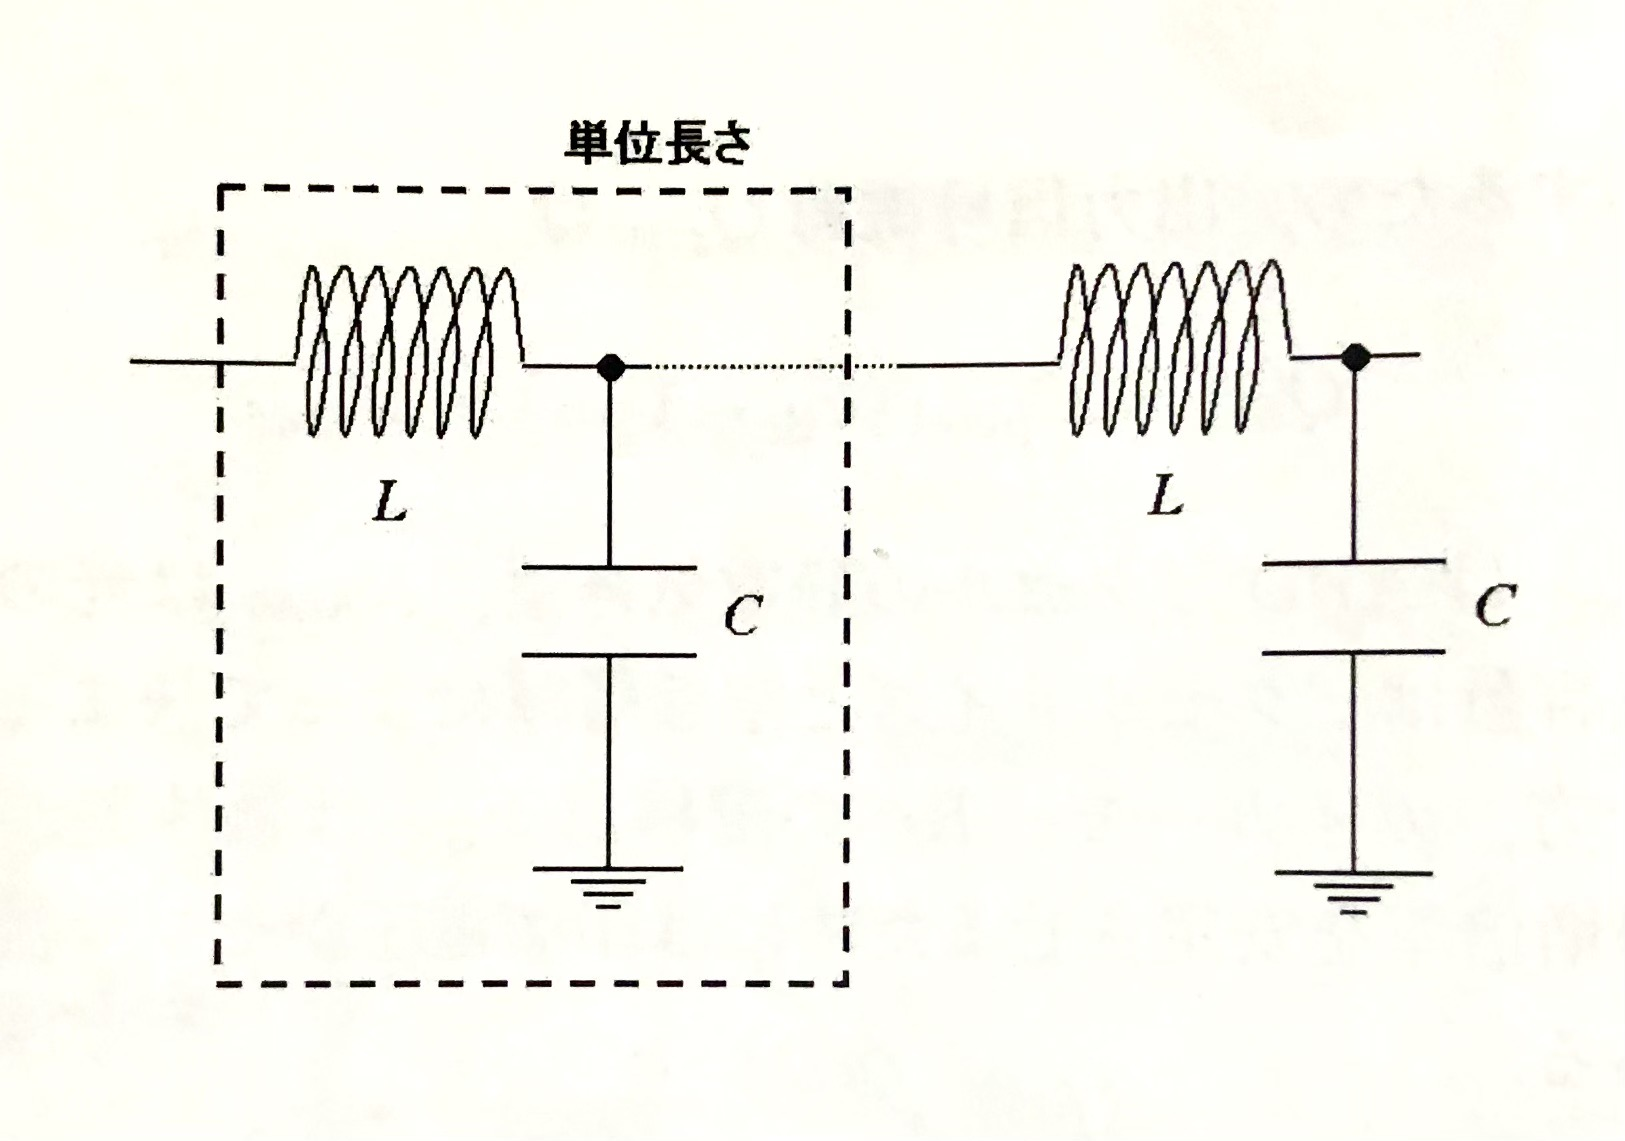
\includegraphics[width=10cm]{./assets/circuit.jpg}
  \caption{同軸ケーブルの等価回路}
  \label{fig:circuit}
\end{figure}
\begin{align}
  \Delta V & = -\Delta z L\diffp{I}{t} \\
  \Delta I & = -\Delta z C\diffp{V}{t}
\end{align}
これより極限を取ると次の微分方程式が成り立つ。
\begin{align}
  \diffp{V}{z} & = -L\diffp{I}{t} \\
  \diffp{I}{z} & = -C\diffp{V}{t}
\end{align}
よって電圧 $V$ について波動方程式が求まる。
\begin{align}
  \diffp[2]{V}{z} = -L\diffp{I}{z,t} = LC\diffp[2]{V}{t}
\end{align}
この一般解については次のようになる。
\begin{align}
  V(z, t) & = \int_0^\infty\dl{k}\ab(V_+(k)e^{ik(z - vt)} + V_-(k)e^{ik(z + vt)}) \\
  I(z, t) & = \int_0^\infty\dl{k}\ab(I_+(k)e^{ik(z - vt)} + I_-(k)e^{ik(z + vt)})
\end{align}
この進行波について上の微分方程式より次のような関係式が成り立つ。
\begin{align}
  ikV_+(k)              & = i\omega LI_+(k)                                              \\
  i\omega CV_+(k)       & = ikI_+(k)                                                     \\
  \frac{V_+(k)}{I_+(k)} & = \frac{\omega L}{k} = \frac{k}{\omega C} = \sqrt{\frac{L}{C}}
\end{align}
これはこの回路の特性インピーダンスを示す。

T コネクタについては同軸ケーブルの特性インピーダンスと同じインピーダンスを持つ抵抗または回路を並列にすべての終端に置くことで全体として反射を防ぐことができると思われる。


\subsection{授業の感想}
物理学実験 B で光電子増倍管やシンチレータ、半導体によるセンサといった実験装置や回路などによる観測技術については一通り学んでいたのでそれを少し応用するだけで実験が出来た。
こうして実験することでさまざまな概念がちゃんと紐づくような感じがして面白かったです。
ただレポートを書いているときに他の実験の文献を漁っているとそれを更に応用して様々な実験を行っていてもう少し応用のある実験でも良さそうと思いました。

\section{参考文献}
\begin{itemize}
  \item 宇宙線ミューオンの観測 \url{https://www-he.scphys.kyoto-u.ac.jp/gakubu/A1/reports/a1report16b.pdf}
\end{itemize}

\end{document}